%!TEX root = ../thesis.tex
%Adding the above line, with the name of your base .tex file (in this case "thesis.tex") will allow you to compile the whole thesis even when working inside one of the chapter tex files
%: ----------------------- introduction file header -----------------------
\singlespacing
\chapter{Introduction}
\label{chap:1}
\vspace{-8mm}
\doublespacing
The Sun has long been the focus of humanity's curiosity. Throughout history it has been the harbinger of new religions, philosophies, and sciences. It has changed our understanding of our place in the Universe and allowed us to push forward the frontiers of stellar astronomy. Although our understanding of the Sun is nowadays more advanced, the curiosity we hold for it has not changed since the very early humans.
Now, we understand the Sun is a star similar to any other in its class, currently going through a relatively unchanging 11 year cycle of activity that is extremely rich in physical complexity. The study of such complex phenomena has yielded immeasurable advances in many areas of physics such as spectroscopy, plasma physics, magnetohydrodynamics (MHD), particle physics, to name but a few. Although some of these sciences have grown over decades (or even centuries) they are still incomplete. I hope this theses will contribute to the continuing growth of these sciences and to the understanding of our nearest star.
\clearpage	
%Here is the introduction of the thesis, complete with a few references  \citep{sagan1997demon, prothero2007evolution}.  Section \ref{sec:1} contains Equation \ref{eqn:1}, Section \ref{sec:2} has Figure \ref{fig:1} and Section \ref{sec:3} has Table \ref{tab:1}. Chapter \ref{chap:2} has pretty much nothing in it.
\noindent
This chapter will begin with a short introduction to the basic physical concepts governing the behaviour of the Sun, including the layers of solar interior and atmosphere. This will be followed by an overview of both the historical and state-of-the-art observational results of coronal mass ejections and coronal shock research. I will finish by highlighting open questions in the field and give a thesis outline for addressing these questions.

\section{The Sun}\label{sec:1}

The Sun is our nearest star, located $1.49\times10^6$\,km from Earth at the centre of our solar system. Located on the main sequence of the Hetzpring-Russel (HR) diagram, it has a spectral class of G2V, with a luminosity of $L_{\odot}=(3.84\pm 0.04)\times10^{26}$\,W, mass of $M_{\odot}=(1.9889\pm0.0003)\times10^{30}$\,kg and radius of $R_{\odot}=(6.959\pm0.007)\times10^8$\,m \citep{foukal2004}. It was born approximately $4.6 \times 10^9$\,years ago when a giant molecular cloud underwent gravitational collapse and began hydrogen nuclear fusion at its core \citep{montmerle2006, bouvier2010}. The energy produced from this fusion resulted in enough pressure to counteract gravitational contraction and bring about a hydrostatic equilibrium, allowing the young star to reach a stability that is sustained today. It is estimated the Sun will maintain this stability for another 4.8 billion years from present time, at which point, it will move off the main sequence and into a red giant phase \citep{sackmann1993}. During this later part of its life, begin nuclear burning of heavier elements such as helium, carbon and oxygen and it will grow in size to 200 times its current radius. Once carbon burning in the core has ceased it can no longer sustain nuclear fusion of heavier elements, resulting in a gravitational instability that will eventually lead to a stellar nova. This nova will result in the loss of the outer envelopes and ultimately the Sun's death, leaving behind a compact and dense white-dwarf.

Until such time, the Sun will remain on the main sequence in a regular state of hydrogen fusion in its core. The energy released during this process is the ultimate source of light and all energetic activity that we observe from Earth and beyond. Before we can understand how this energy manifests in the solar atmosphere as a variety of energetic phenomena, it is important to understand how the energy is generated and transported through its interior and finally released into its atmosphere and interplanetary space.

\subsection{Solar Interior}\label{sec:10}

The theoretical treatment of how the solar interior is structured and how it behaves it through the \textquoteleft standard solar model' or SSM. The SSM is a grouping of theories that described how the Sun was formed, how it maintains its stability, how it generates energy, and how this energy is transported through its interior and released at the surface. Much of the major developments of this theory have been in the 20th century, due mainly to the pioneering experiments in solar neutrino physics and helioseismsology. Hence, the development of the SSM has mainly been through a refinement of the theory based on these observational fields. Although the SSM has increased in sophistication, its four main aspects remain the most general framework for describing the behavior of the solar interior.

The SSM firstly states that the Sun was born from the gravitational collapse of a primordial gas of hydrogen, helium, and traces of other heavy elements \citep{sackmann1993}. Secondly, it maintains its structural stability via a hydrostatic equilibrium such that the gravitational force is balanced by a pressure gradient ($\grad{P}=-\rho g$) at each radial distance inside the star. The third main aspect of the SSM involves the source of the Sun's energy. Much of the early ideas proposed during the 19th century involved some form of chemical reaction or energy released during a slow gravitational contraction \citep{shipley2001}. However, during the first half of the 20th century the theory that the Sun is at least as old as the Earth began to come into focus. A solar age of at least 4.5 billion years prompted the question of what energy source could sustain the Sun's luminosity for such a length of time? Amongst the various suggestions was thermonuclear fusion, and, as a result, it should be possible to observe the neutrino products of this fusion process. Hence, in the 1960s, a number of pioneering neutrino physics experiments were developed in an attempt to detect solar-generated neutrinos at Earth. These pioneering experiments, as well as there more sophisticated counterparts today, confirm much of the theories of nuclear fusion as the source of the Sun's energy \citep{davis1968}.

From the 1970s onwards there has been a confirmed detection of neutrinos generated in a hydrogen fusion process, namely the proton-proton or `pp' chain, in the solar core. In this process, four protons are fused to form a helium nucleus. This can occur in a variety of ways, but at the Sun's core temperature of 15 MK, the dominant reaction is the pp\,I chain given by
\begin{eqnarray}
^{1}_1\mathrm{H} + ^{1}_1\mathrm{H} \rightarrow ~^{2}_1\mathrm{H} + e^{+}  + \nu_e \\
%
^{2}_1\mathrm{H} + ^{1}_1\mathrm{H} \rightarrow ~^{3}_2\mathrm{He} + \gamma \\
%
^{3}_2\mathrm{He}+^{3}_2\mathrm{He} \rightarrow ~^{4}_2\mathrm{He} + 2^{1}_1\mathrm{H}
\end{eqnarray}
where $^{1}_1\mathrm{H}$ is a hydrogen nucelus, $^{2}_1\mathrm{H}$ is deuterium, $^{3}_2\mathrm{He}$ is tritium, $^{4}_2\mathrm{He}$ is helium, $e^{+}$ is a positron, $\nu_e$ is an electron neutrino, and $\gamma$ is a gamma ray photon. Reactions (1.1) and (1.2) must happen twice for (1.3) to occur. Taking this into account, the entire process may be summarised as 
\begin{equation}
4 ^{1}_1\mathrm{H}  \rightarrow ~^{4}_2\mathrm{He} + 2e^{+} + 2\nu_e + 2\gamma
\end{equation}
liberating $4.2\times10^{-12}$J of energy per reaction, with $\sim$2.4\% of the energy carried away by the neutrinos. This particular form of the pp-chain (pp\,I) occurs in 86\% of the cases in solar core nuclear fusion \citep{turk2011}. However, there are other reactions capable of producing He from H catagorized into pp\,II, pp\,III etc, which each involve production of $^7_4$Be and $^8_5$B, which were actually the first to be confirmed despite these reactions being less common that pp\,I \citep{davis1968}. 
%The initial neutrino detections at Earth were the result of the pp III reaction which involves the creation of $^8_5$B, followed by a decay to $^8_4$Be, a positron, and an electron neutrino \citep{davis1968}. 
%These early detections and the results of more recent experiments such as the SuperKamiokande \citep{fukuda1998} show that the expected neutrino flux given by the standard solar model is smaller than the observed flux. This deficit in neutrino flux observations became the famed `solar neutrino problem' during the 1970s. 
%One of the proposed explanations for the neutrino deficit was via an oscillation of the neutrino amongst three sets of `flavors' i.e., the neutrino can be either an electron $\nu_e$, muon $\nu_{\mu}$, or tau $\nu_{\tau}$ neutrino, of which only one flavor was detected.
%With the original detectors only being able to detect the $\nu_e$, this would result in a flux deficit (non-detection of $\nu_{\mu}$ and $\nu_{\tau}$). 
%This oscillation amongst three flavors was given the name the `MSW effect' after \citet{mikheev1986} and \citet{wolfenstein1978}, and later confirmed experimentally by the SuperKamionkande experiment.

The neutrino experiments together with the SSM provide much of what we know about the solar energy generation and the solar core. They imply a temperature of $15.6\times10^6$\,K and density of $1.48\times10^5$\,kg\,m$^{-3}$ at solar centre, where energy generation is via fusion which occurs $0.0-0.25\,R_{\odot}$ (Figure~\ref{fig:solar_atmosphere}). This range in heights defines the solar core and outside this range the temperature drops to a value low enough for the cessation of fusion. While thermonuclear fusion and the generation of solar energy is the third aspect of the SSM, the fourth aspect involves exactly what happens to this energy once it is generated i.e., it describes an energy transport mechanism.
%, and also confirm the existence of a variety of pp reactions (pp 1 to pp IV), and some level of Carbon-Nitrogen-Oxygen (CNO) fusion process. 
%These fusion processes occur over $0.0-0.25\,R_{\odot}$ (Figure~\ref{fig:solar_atmosphere}), which defines the solar core. Outside the core the temperature drops to a value such that fusion ceases. While thermonuclear fusion is the third aspect of the SSM involves the generation of solar energy, the fourth aspect involves exactly what happens to this energy once it is generated i.e., it describes an energy transport mechanism.


Beyond $0.25\,R_{\odot}$ the temperature drops to 8\,MK, such that fusion stops but only free protons and electrons exist. In this environment, the photons continuously scatter off free particles, undergoing a random walk toward the surface over a distance of $0.25-0.7\,R_{\odot}$. This region is known as the radiative zone and has densities of $2\times10^4-2\times10^2$\,kg\,m$^{-3}$, resulting in a small photon mean free path (mfp) of $9.0\times10^{-4}$\,m. The photons proceed towards the solar surface over a very long time scale, taking on the order of $10^{5}$ years to traverse this region \citep{mitalas1992}. The occurrence of such a radiative energy transport results in a temperature gradient given by 
\begin{equation}
\frac{dT}{dr} = -\frac{3}{16 \sigma}\frac{\kappa \rho}{T^3}F_{rad}
\end{equation}
%Note the above equation is actually a diffusion equation for radiation. Take the divergence of both sides and you have $\grad\dotF = \kappa^'\grad^2 T$, with $\kappa^'$ being the diffusion coefficient given by $\kappa^i=\frac{16\pi\sigmaT^3}{3\kappa \rho}$ e.g., the opacity controls to mean free path, and hence the diffusion of photons.
where $\sigma$ is the Stefan-Boltzman constant, $\kappa$ is the mass extinction coefficient (opacity per unit mass), $\rho$ is mass density, $T$ is temperature, and $F_{rad}$ is the outward radiative flux \citep{foukal2004}. This implies that for a particular outward flux, if the opacity increases, a steeper temperature gradient is required to maintain such a flux. At $0.7\,R_{\odot}$ the temperature drops to 1\,MK allowing protons to capture electrons into a bound orbit. The existence of electrons in atomic orbit results in a dramatic increase in opacity of the plasma \citep{turk2011} and hence the temperature gradient increases. The increased temperature gradient required to sustain the energy flow may lead to the onset of a convective instability beyond $0.7\,R_{\odot}$ toward the solar surface. This instability will occur if the temperature gradient in the star is steeper than the adiabatic temperature gradient 
\begin{equation}
\Bigg|\frac{dT}{dr}\Bigg|_{star} > \Bigg|\frac{dT}{dr}\Bigg|_{adiabatic}
\end{equation}
This is known as the Schwarzchild criterion, and it is fulfilled from $0.7-1\,R_{\odot}$ $-$a region known as the convection zone. The temperature and density drop as height increases and finally reaches T$\sim$$6000$\,K and mass densities of $\rho\sim1\times10^{-5}$\,kg\,m$^{-3}$. Although no complete theoretical treatment of convection exists, mixing length theory and hydrodynamical modeling are used to determine how convection occurs in the solar interior. Convection ceases at $1\,R_{\odot}$, where the environment makes a sudden transition to convectively stability. At this point the opacity drops and energy is released in the form of radiation, demarcating the start of the solar surface, known as the photosphere. 
\begin{figure}[!t]
\begin{center}
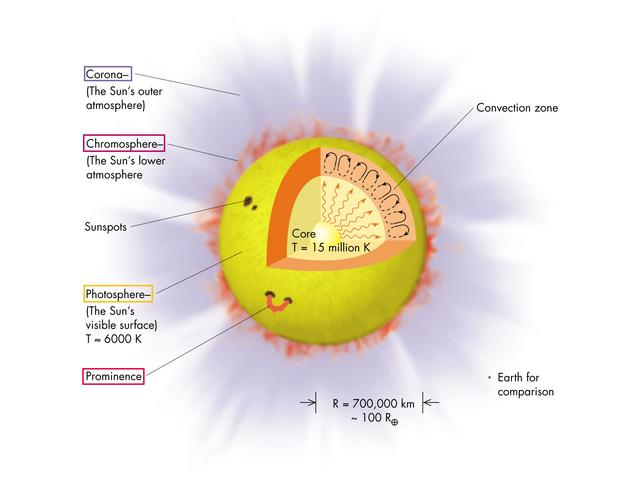
\includegraphics[trim = 0cm 0.5cm 0cm 0cm, width=0.8\textwidth]{images/solar_atmosphere}
\caption[The solar interior and atmosphere]{The structure of the solar interior and atmosphere, including the core, radiative zone, convective zone, photosphere, chromosphere, and corona.  While the various interior zones are demarcated in terms of the dominant energy transport mechanism, the layers of the solar atmosphere are usually demarcated by temperature changes as height above the solar surface increases. The temperature ranges from $\sim$6000\,K in the photosphere to above 1\,MK in the corona.}
\label{fig:solar_atmosphere} 
\end{center}
\end{figure}

% Yuhong Fan, Living Reviews. "Because of the rapid decrease of the various scale heights in the top layer of the solar convection zone which demands increasing numerical resolution, it is not yet feasible to perform 3D MHD simulations that extend from the bottom of the convection zone all the way to the photosphere."

Much of what we know about the depth, temperature, and density of the convection zone comes from a fine-tuning of the standard solar model, such that the model reproduces observational properties of neutrino experimaents and the field of helioseismology. Helioseismology makes use of the fact that the Sun acts as a resonator for acoustic waves which manifest as detectable oscillations in the doppler shift of photospheric Fraunhofer lines. These acoustic waves are referred to as pressure or p-modes, and a variety of wavelengths exist, generally with a period of approximately 5 minutes \citep{turk2011}. 

\begin{figure}[!t]
\begin{center}
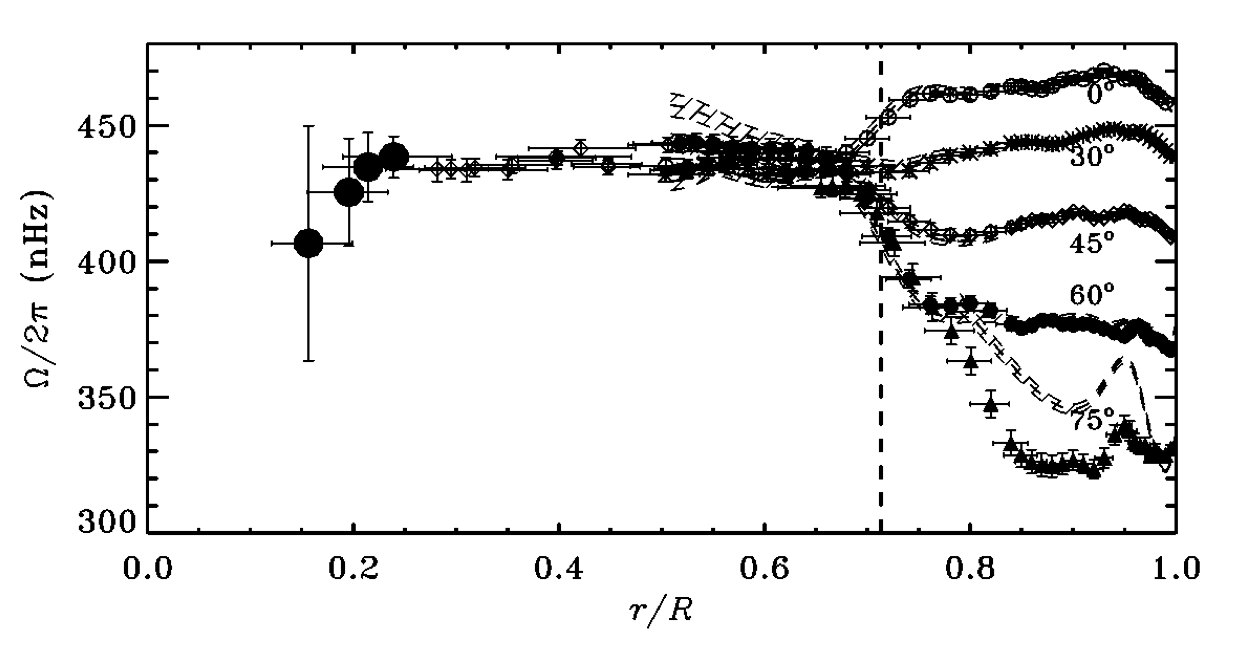
\includegraphics[trim = 0cm 0.5cm 0cm 0cm, width=0.8\textwidth]{images/differential_rot.png}
\caption[Differential rotation rate as a function of latitude and depth]{Helioseismological determination of interior rotation rate in nanoHertz (nHz) as a function solar radius, starting from solar centre ($r=0.0$) to surface ($r=1.0$). The separate symbols show different latitudes, from $0^{\circ}$ to $75^{\circ}$. The data show that the interior rotates differentially down to $\sim$$0.7\,R_{\odot}$. The dashed line demarcates the boundary between solid body rotation and differential rotation. The transition from solid body to differential rotation occurs in a highly sheared layer known as the tachocline, a very important layer for solar magnetic field generation \citep{thompson2003}.}
\label{fig:diff_rot} 
\end{center}
\end{figure}

The shorter wavelengths in the mode propagate into the solar convection zone and experience a total internal reflection at a shallow depth, while longer wavelengths can penetrate into much deeper layers. Hence depending on the period observed, the oscillations provide a probe of the dynamical properties at a particular depth inside the sun. Analysis of these oscillatory modes has revealed that the differential rotation that is observed at the solar surface continues down into the convection zone, however the deeper radiative zone rotates as a solid body (Figure~\ref{fig:diff_rot}). In going from the convection zone to the radiative zone there is a sudden dramatic transition in the rotational dynamics of the solar interior \citep{thompson2003}. This sudden change occurs in a region sandwiched in between the radiative and convective zones, known as the tachocline. The study of this layer is extremely active as it is believed to play an important role in the generation and evolution of the solar magnetic field.


%Once such property closely monitored is the sound speed, which is seen to match the predicted sound speed based on the standard model. However, the observation and prediction show the biggest deviation at a depth of $0.3\,R_{\odot}$, which is the region where the radiative zone transitions to the convective zone. This obviously implies that SSM is lacking in its description of how the solar interior is stratified at this depth. This partly due to the fact the SSM does not take into account differential rotation. The solar surface rotates faster at the equator than it does at the poles i.e., angular velocity is stratified with latitude. Helioseismology has revealed that such differential rotational continues to the bottom of the convection zone. In the deeper radiative zone and core the Sun rotates as a solid body see Figure~\ref{fig:diff_rot}. There is a dramatic change in the internal dynamics when transitioning from convective to radiative zones. 

%As predicted by sound speed measurements and differential rotation, the region sandwiched in between radiative and convective zones is and extremely important boundary. It is known as the tachocline, and the dynamics of this thin layer is believed to play and extremely important role in the generation and evolution of the solar magnetic field \citep{thompson2003}.

\subsection{Solar Magnetic Field and Dynamo}\label{sec:dynamo}

The solar magnetic field plays a dominant role in the energetic activity occurring in the solar atmosphere. At solar activity minimum the solar magnetic field has a poloidal dipolar structure, with the polar axes generally being coincident with the rotational axes. However as the activity cycle progresses towards a maximum, the field gains a strong toroidal component, making it far more dynamic and complex. This complex toroidal component manifests at the surface as sunspots, hence the number of sunspots on disk has been used as a proxy for the activity cycle for over 100 years, often showing an approximate 11 year periodicity (Figure~\ref{fig:butterfly}, bottom panel). At the beginning of the cycle sunspots tend to appear on disk with a latitudinal distribution of $\pm30^{\circ}$ of the equator. As the cycle progresses, sunspots appear at lower and lower latitude (known as Sp\"{o}rer's law), until they eventually disappear at the end of a cycle. Sunspot latitude with respect to time is shown in Figure~\ref{fig:butterfly}, top panel, and is known as the `butterfly diagram'.

Sunspots in there simplest case emerge as a dipoler structure, with the leading spot being closer to the equator, such that the dipole is titled relative to the solar equator (Joy's law). In a given hemisphere, the leading sunspot and trailing spot have opposite polarities, with the polarities reversed in the other hemisphere (Hayle's law). The trailing polarity can often be more fragmented and dispersed than the leading polarity. Despite sunspots generally having a dipolar structure, spot groups can be far more complex, having a complex multipolar structure -- these spots are usually the more active.

Over the course of a solar cycle, the sun changes polarity (at the time of sunspot maximum). For example, an overall dipolar configuration of North-South will become South-North, another cycle will bring it back to North-South once more. While the activity cycle usually last 11 years, one full magnetic cycle has a period of 22 years. The complex behavior of the solar magnetic field over an 11 year activity cycle, during which the dipole reverses sign, is generally explained by solar dynamo theory. The theory employs magnetohydrodynamic (MHD) models that involve large-scale flow patterns of the solar interior that act to both induct and diffuse the magnetic field such that it produces the familiar 11 year magnetic activity cycle \citep{charbon2010}. 


\begin{figure}[!t]
\begin{center}
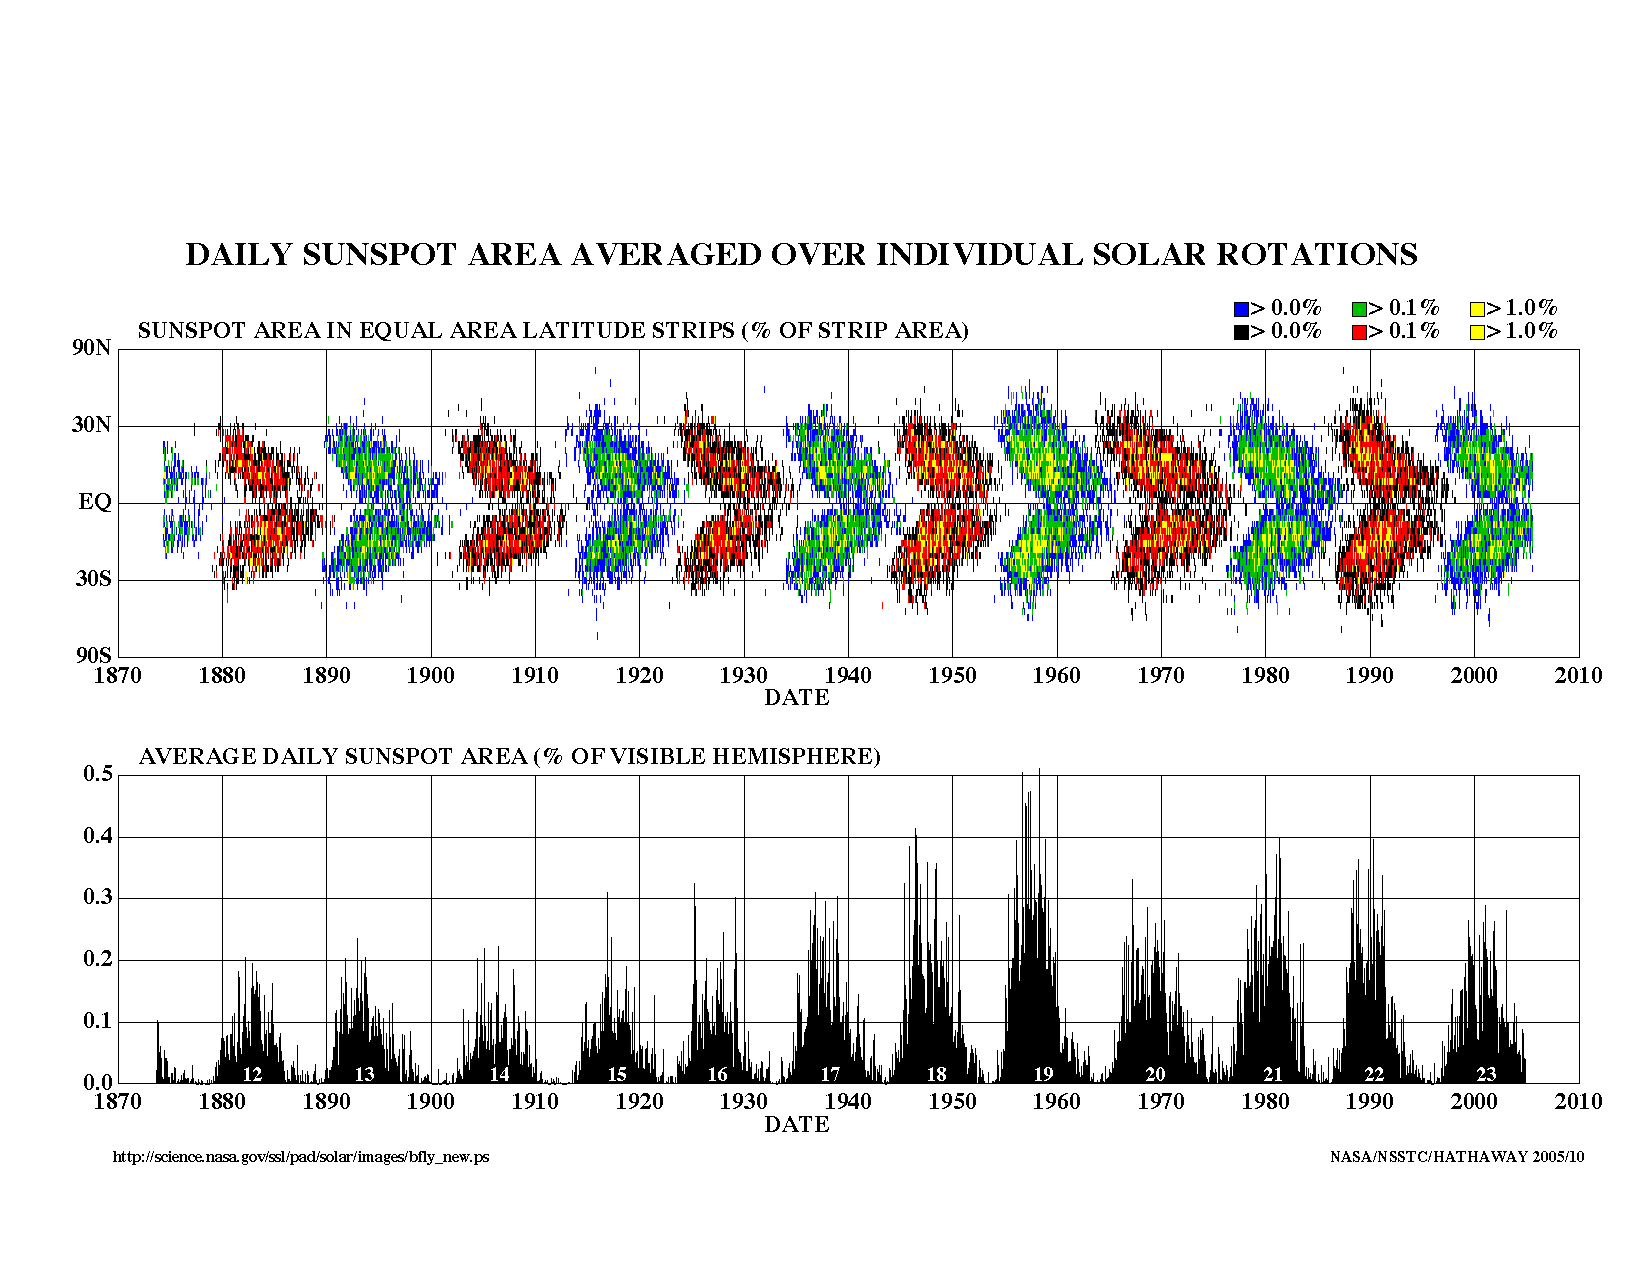
\includegraphics[scale=0.55, trim =1cm 2cm 0cm 3cm]{images/bfly_new.pdf}
\caption[The solar butterfly diagram]{Top: The latitude of sunspots as a function of time. During the rise phase of each cycle the sunspots have a latitudinal distribution of $\pm30^{\circ}$ from the equator.  As the solar cycle progresses, sunspots emergence takes place at an increasingly lower latitude. Bottom: Sunspot area as a function of time. The spot area, or number of spots, is a proxy for solar magnetic activity which approximate follows and 11 year periodicity.}
\label{fig:butterfly} 
\end{center}
\end{figure}
\begin{figure}[!h]
\begin{center}
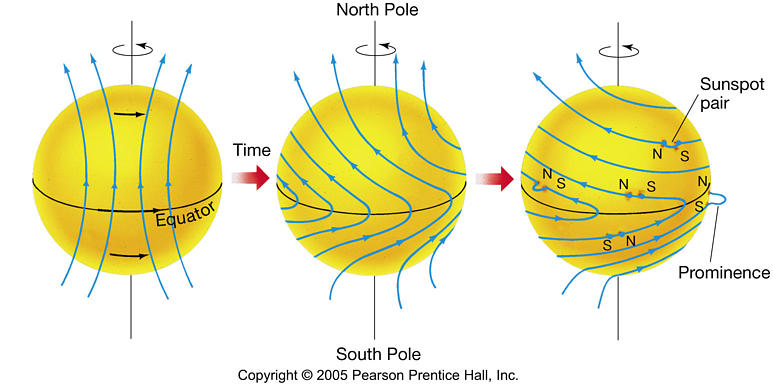
\includegraphics[]{images/Babcock}
\caption[The Babcock model of magnetic field evolution in the Sun]{Differential rotation and flux freezing result in the poloidal dipolar magnetic field, generated by dynamo action, to be dragged around in a toroidal direction, an action known as the omega effect. Buoyancy of the field lines results in them rising and twisting, known as the alpha effect, eventually surfacing to become bipolar fields that extend far into the corona.}
\label{fig:Babcock} 
\end{center}
\end{figure}

%The complex behavior of the solar magnetic field over an 11 year activity cycle, during which the dipole reverses sign, is generally explained by solar dynamo theory. This is a magnetohydrodynamic theory that involves large-scale flow patterns of the solar interior that act to both induct and diffuse the magnetic field such that it produces the familiar 11 year magnetic activity cycle and other observed phenomena (Sp\"{o}rer's, Joy's, and Hale's laws). The theory is incomplete but there is an accepted paradigm on the general behaviour of the magnetic field throughout the cycle, known as the Babcock model.

%Magnetohydrodynamics (MHD) is employed to describe such that the magnetic induction equation and velocity field equation (equation of motion) are solved in numerical models to produce a toroidal field from a poloidal one, a process known as the $\Omega$-effect. The theories must adhere to the constraints provided by observations of the sunspot cycle (Sp\"{o}rer's, Joy's, and Hale's laws), and also helioseismology observations of how the interior is structured.

Although solar dynamo theory is an active area of research and a number of questions still remain, the generally accepted paradigm for the activity cycle was first proposed by \citet{babcock1961}. The mechanism involves differential rotation of the solar convection zone tends (Figure~\ref{fig:diff_rot}) that tends to drag the field from a poloidal position into a toroidal one (known as the $\Omega$-effect), eventually winding the field around the solar axis into a a stressed state, see Figure~\ref{fig:Babcock}. The main storage of this wound field is in the region below the convection zone known as the tachocline. This region has an `overshoot' layer, in which descending convective flows are a trapped due the subadiabicity of the region (convectively stable). This stability allows field to be built up and stored into complex magnetic structures that may form twisted `flux-ropes' due to the continuous wrapping of the field during the $\Omega$-effect. Due to the rope's excess magnetic pressure, it becomes convectively unstable and begins to rise and experience a Coriolis force that induces a tilt of the rope with respect to the equatorial plane (this is known as the $\alpha$-effect and is an explanation of Joy's law). The field eventually surfaces creating sunspots in the photosphere and a complex magnetic structure in the solar atmosphere known as an active region \citep{fan2009}. The active regions themselves may be sheared, twisted and generally evolves to build huge amounts of potential energy. The release of this potential energy plays a big role in the dynamics of the solar atmosphere.


%Dynamo theory attempts to explain this $\alpha\Omega$-effect wrapping and build up of toroidal flux in the solar interior via inductive plasma flows \citep{charbon2010}, particularly using the observed flow structure from helioseismology. MHD convective instabilities is employed to describe the $\alpha$-effect rise of flux systems from the stably convective tachcoline/overshoot layer into the solar atmosphere \citep{fan2009}. 


\subsection{Solar Atmosphere}\label{sec:12}

The solar atmosphere begins above the visible surface of the sun, known as the photosphere. At this point, the Sun become optically thin to visible radiation and light escapes from this surface. Beyond this visible surface is the solar chromosphere, and the corona, which eventually becomes the solar wind. Each of these layers is home to a complex variety of phenomena, and each layer, with its accompanying attributes, is described here.


\subsubsection{Photosphere}\label{sec:121}

As mentioned, the photosphere begins where the atmosphere become optically thin to visible radiation. \textquoteleft Visible light' in this instance is usually taken to mean light with a wavelength of 5000\,\AA, hence the emergent light from the photosphere is taken to come from the surface at which $\tau_{5000}=2/3$, where $\tau$ is the optical depth. The optical depth of 2/3 is a consequence of the Eddington-Barbier approximation, and says that emergent flux $F_{\nu}$ from the photosphere is given by

\begin{equation}
F_\nu = \pi B_\nu(\tau=2/3)
\end{equation}
e.g., the emergent flux is given by $\pi$ times blackbody intensity at an optical depth of 2/3, where blackbody intensity $B_\nu$ is given by Planck's law 
\begin{equation}
B_\nu = \frac{2h\pi\nu^3}{c^2}\frac{1}{\mathrm{exp}(h\nu/k_BT)-1}
\label{eqn:planck}
\end{equation}
where $h$ is Planck's constant, $\nu$ is frequency, $c$ is the speed of light, $k_B$ is Boltzmann's constant, and $T$ is temperature. Integrating equation~\ref{eqn:planck} over frequency this results in $F = \sigma T^4(\tau=2/3)$, shoqing the frequency integrated flux is proportional to the temperature at $\tau=2/3$, hence the effective temperature of solar blackbody radiation is $T_{eff}=T(\tau=2/3)=5800$\,K. Solar radiation at visible wavelengths is most closely characterised by a blackbody of temperature 5800 K, although the brightness temperature $T_B$ of the photosphere can deviate from this value, since not all frequencies emerge from the same optical depth.

The visible appearance of the photosphere reveals a small scale granular structure, with granules of typical size scale of 1000\,km and a lifetime of 5--10 minutes. The granules typically show bright centers surrounded by darker intergranular lanes. Doppler measurements reveal that granule centres have a positive (upward) velocity of up to $\sim1$\,km\,s$^{-1}$, with intergranular lanes having a negative (downward) velocity. Such upward and downward flow indicates that granulation at the photosphere is the surface manifestation of convective activity in the deeper layers of the interior, although the size scales of granules are much smaller than the convective plumes believed to permeate the convection zone \citep{schrijver2008b}. As well as the conspicuous granulation at the photospheric surface there is also a much larger scale \textquoteleft super-granulation' which has much the same mechanism as the granules e.g, upflows at granule centre and downflows at the edges in the granular network. The flow speeds are much slower with typical speeds of $0.1$\,km\,s$^{-1}$, and they have a much larger size of $10,000-30,000$\,km with lifetimes of several days. They have an important role in the build up and concentration of magnetic flux in the intergranular lanes. Apart from granules and supergranules, the most conspicuous features of the photosphere are sunspots. As discussed in Section~\ref{sec:dynamo}, these are the surface manifestation of concentrated magnetic flux that has penetrated from the solar convective zone into the solar atmosphere. The spots have a temperature of $\sim$4000\,K, which is cooler than the typical solar blackbody temperature of $5800$\,K. Typical magnetic field strengths in sunspots are on the order of kilo-Gauss, while quiet regions are permeated by fields with tens of Gauss.


The temperature and density profile of the photosphere is usually determined through an analysis of the emission and absorption lines of a variety of elements and their ionization species. Dark absorption features, known as Fraunhofer lines, are superimposed on the photospheric blackbody and provide a useful diagnostic of temperature with respect to height. The most notable of the Fraunhofer lines are the H$\alpha$ and Ca\Rmnum{2} H and K lines. These lines, as well as others, are used in the models of \citep{vernazza1981, fontenla1988, gabriel1976}, whereby a model temperature and density profile of the solar atmosphere is used to calculate the emergent line intensity, using radiative transfer theory. This temperature and density profile is adjusted until the the modeled emergent intensities match the observed ones. The results of this these models is shown in Figure~\ref{fig:val}. After the $\tau_{5000}=1$ level the temperature drops to a minimum of $\sim$4400\,K at $\sim$400\,km above the photopshere before rising again, eventually undergoing a rapid increase at $\sim$2000\,km. The region between the temperature minimum up the height at which temperature begins to rise rapidly is the next layer of the atmosphere beyond the photosphere, known as the chromosphere\footnote{These boundaries can vary, depending on the phenomenon observed e.g., spicules are chromospheric phenomenon which can extend far beyond the upper boundary of $\sim$2000\,km}. 

%About 15% of photospheric opacity is attributed to absorption features. The rest is H- opacity

\begin{figure}[!t]
\begin{center}
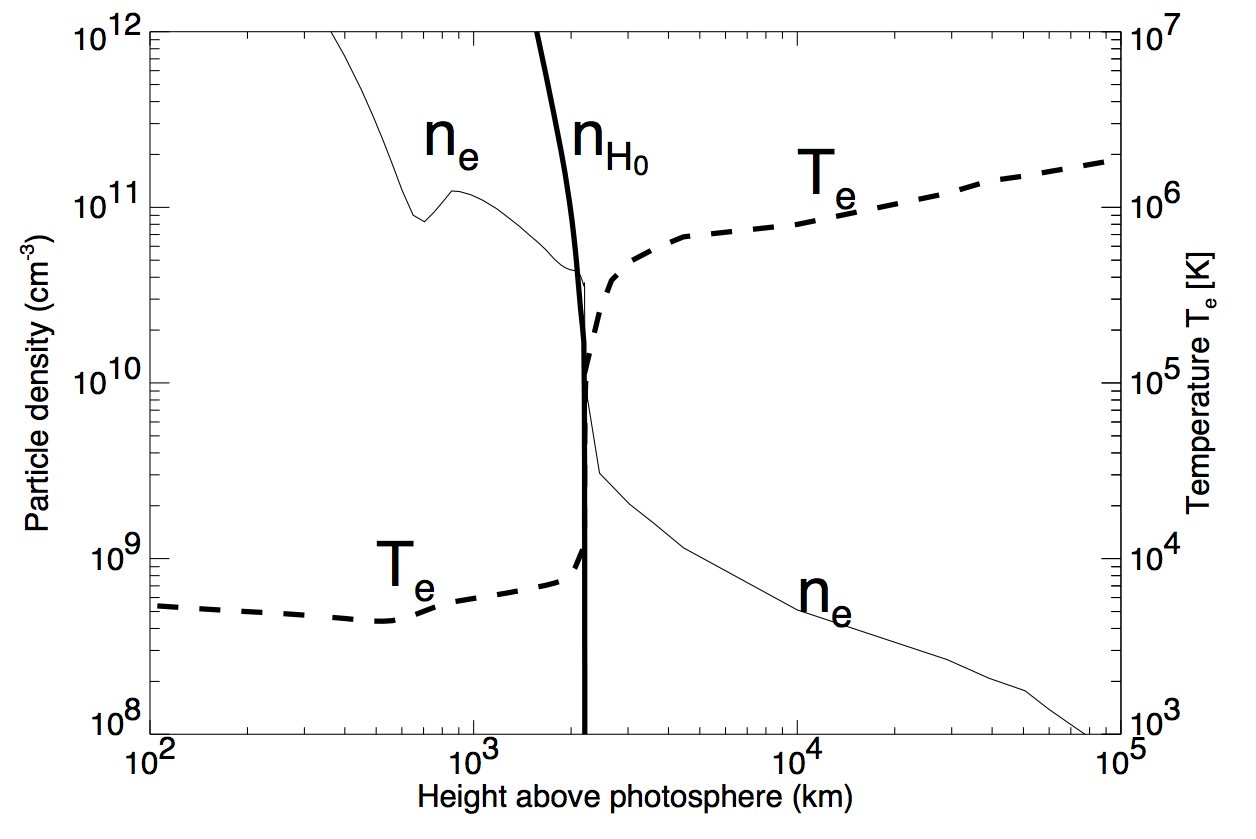
\includegraphics[scale=0.3]{images/FAL-C.png}
\caption[The temperature and density as a function of height above the photosphere]{Temperature and density variation in the solar atmosphere constructed from the models of \citep{vernazza1981, fontenla1988, gabriel1976}, adopted from \citep{phillips2008}.}
\label{fig:val} 
\end{center}
\end{figure}


\subsubsection{Chromosphere}\label{sec:122}

As predicted by the models of \citep{vernazza1981, fontenla1988, gabriel1976}, at $\sim$400\,km above the $\tau_{5000}=1$ surface the temperature drops to a minimum of $\sim$4400\,K. Beyond this minimum the temperature begins to rise again, demarcating the beginning of the chromosphere. This layer of the atmosphere is generally accepted to extend to a height at which temperatures reach 20,000\,K, however temperatures as high as $\sim$$1\times10^5$\,K are sometimes attributed to chromospheric heights, hence it is observable at ultraviolet (UV) wavelengths as well as visible. 

%The chromosphere is primarily observed through the the Fraunhofer H$\alpha$ and Ca\Rmnum{2} H and K lines. These lines in particular provide a good diagnostic of the chromospheric environment over a large height range since different sections of the lines are formed over various heights. By viewing the sun at or near the cores of the lines we may view different height s in the chromospheric part of the atmosphere. The chromosphere, when observed using the Ca lines, shows a highly non-uniform structured and structured appearance. The structure is made up of dark cells with a diameter of approximately 30,000\,km, with bright boundaries of the cells making up a network of bright features known as \textquoteleft the chromospheric network'. These network boundaries consisting of bright points are positions of near vertical magnetic field with a strength of 10\,Gauss. This chromospheric network is directly related to the supergranular structure as observed in the chromosphere i.e., the supergranular flows in the photosphere tend to transport field toward the boundaries of the network where they may coalesce and strengthen. These regions of strong magnetic field facilitate heating in the upper chromosphere and hence show up as regions of enhanced emission (by magnetic acoustic oscillations) in the centers of the Ca\Rmnum{2} K3, for example \citep{mcateer2002}. Enhanced emission in the internetwork regions (supergranule centres) show up as bright points when viewing Ca H2V and are now accepted to be formed by heat of the mid-low chromosphere by acoustic shocks \citep{carlsson1997}
%TAKEN OUT TO REDUCE INTRO SIZE

Beyond the temperature minimum there is a broad temperature plateau between $\sim$$1000-2000$\,km, after which the temperature starts to increase dramatically. Similar to the photosphere, supergranulation is present in the chromosphere, indicating that this layer of the atmosphere is magnetically structured with concentrations or bundles of magnetic fields confined to isolated regions in the intergranular lanes. These concentrations of magnetic field are believed to play a role in chromospheric heating \citep{carlsson1997}. When the temperature reaches 20,000\,K the extremely prominent Ly-$\alpha$ emission line is formed, with a wavelength of 191.5\,nm, and this is accompanied by other prominent ultraviolet lines such as those of C \Rmnum{4}, formed at temperatures of $\sim$110,000\,K. Such high temperatures are generally considered to be outside the range of the chromosphere and are indicative of a thin layer of the atmosphere known as the transition region. 

\subsubsection{Transition Region}
The layer sandwiched in between the chromosphere and the corona is the transition region. It is characterised by temeperatures of $\sim$10$^{5}$\,K and has the steepest temperature gradient in the solar atmosphere and extremely narrow at just 200\,km in width. The SDO/AIA 304\,\AA~image shows the chromosphere and transition region, in which the supergranular network can still be seen. The 171\,\AA~image shows the upper transition region and corona. The network has just about disappeared at this height. As described, the network outlines the magnetic structure of the atmosphere, hence magnetic field goes from ordered and concentrated in the chromosphere to more ubiquitous and complex in the corona, sometimes termed the magnetic `canopy'.

%Acoustic shocks heat the low-mid chromosphere in the internetwork region (supergranule centres) and show up as bright points when viewing Ca H2V lines. But the magnetic bright points (at the network boudnary) in higher altitude lines are thought to be upper chromosphere where MHD waves heat the environment, as evidenced by brightening in Ca K3 core. 

%It seems as though whether it's acoustic or magnetic heating depends on the lines (or position in the line) that we look at. If we see bright points in low altitude lines then is shocks. Bright points in high altitude lines correspond magnetic heating. 

%\begin{itemize}
%\item Appearance, Supergranular Network, Bright Points, Spicules, Filaments, Plage etc.
%\item Emission lines, H-alpha, CaII H \& K. 
%\item Temperature, Density, Opacity.
%\item Magnetic field strength.
%\end{itemize}

%Details in the chromosphere are imaged using the lines of H-alpha and Ca II H and K. These Fraunhofer lines are formed over a large range in heights.

%The H-alpha line is photoelectrically controlled, so the decrease in line intensity is to do with the source function being lower because of a lack of photospheric photons at that height the line centre 'samples

%Ca II  H and K is collisionally controlled so the decrease in line intensity is to do with the source function being lower because of the dropping temperature

%Different regions in the Ca II  H and K lines sample different heights in the photosphere/chromosphere. Tuning imagers to different parts of these lines allows imaging of chromosphere at different heights.

%Chromospheric lines not in the visible are the Mg h and k Fraunhofer lines, also collisionally controlled. There is also the Ly-alpha emission line, formed at 20,000 K, which is optically thin. There is C IV, formed at 110,000 K, at this point we are starting to sample to transition region.


%Note: Fraunhofer lines such as Calcium H and K are not as simple as a case of a cloud of cooler gas absorbing lines from a hot radiations source. The Fraunhofer lines are a consequence of the Eddington-Barbier Approximation i.e., that the emergent intensity is equal to the source function at an optical depth of 2/3. So in the centre of the line the opacity goes up and optical depth 2/3 is higher in the atmosphere where the plasma is cooler. Hence, the line is darker at the centre (due to the smaller source function at the cooler temperature).

\subsubsection{Corona}\label{sec:123}

The outermost layer of the solar atmosphere is known as the solar corona, beginning at $\sim$2500\,km above the photosphere. It has an electron number density of $10^{9}$\,cm$^{-3}$ at its base in quiet regions, decreasing to $10^{6}$\,cm$^{-3}$ at distance of $1\,R_{\odot}$ from the solar surface. The models of \citep{vernazza1981, fontenla1988, gabriel1976} reveal that beyond the transition region ($\sim$2500\,km) the temperature in the corona reaches well over $1\times10^{6}$\,K. Such high temperatures allow the formation of emission features that belong to highly ionized heavy elements, for example Fe\,\Rmnum{9}, up to as high as Fe\,\Rmnum{24}. The presence of these highly ionized species (and many others) show that the corona has temperatures in the $1-2$\,MK range in quiet regions, active regions may exhibit temperatures in the range of $2-6$\,MK, while coronal holes may be lower than 1\,MK. The temperatures of a flaring active region can be even higher than this, reaching tens of mega-Kelvin. The high temperatures and presence of highly ionized species of heavy elements means the corona may be primarily observed in the ultraviolet and X-ray. When viewed at these wavelengths, the corona appears highly structured, showing concentrations of bright loops known as active regions (Fig.~\ref{fig:aia_corona}).
\begin{figure}[!t]
\begin{center}
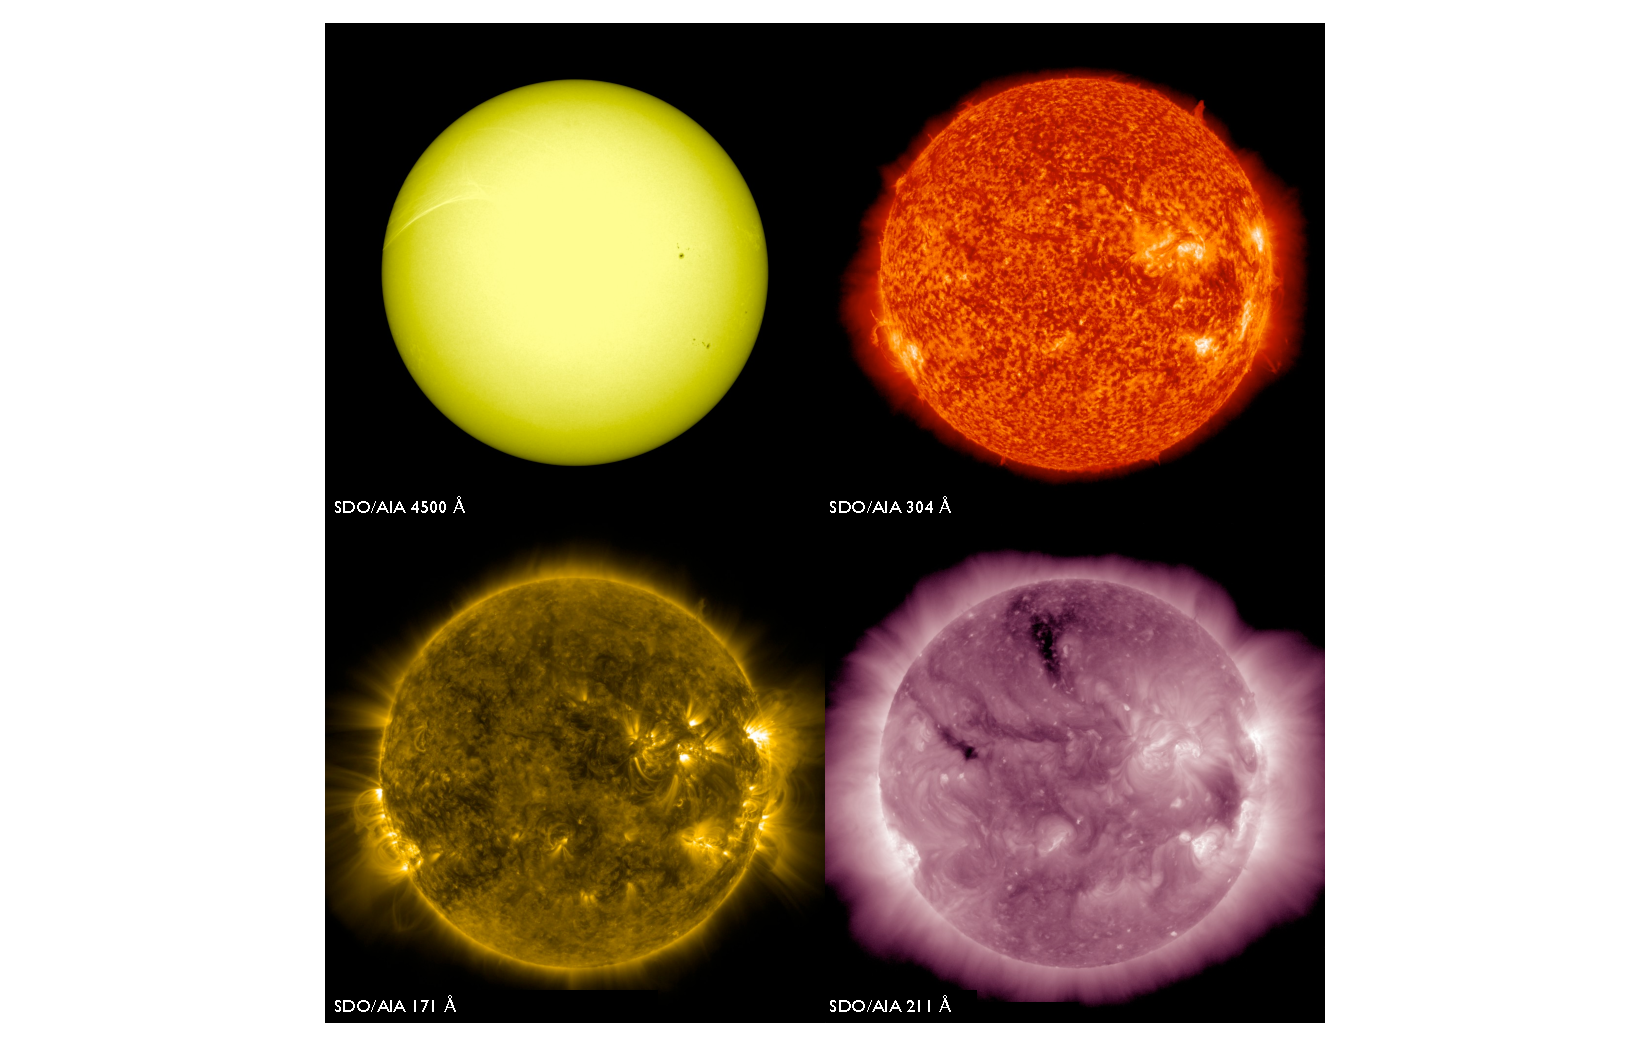
\includegraphics[scale=0.8, trim=5cm 0cm 0cm 1cm]{aia_multi_channel.pdf}
\caption[AIA image of the corona]{Atmospheric Imaging Assembly (AIA) observations of the photosphere (4500\,\AA), chromosphere (304\,\AA), transition region (304\,\AA,171\,\AA), and corona (171\,\AA, 211\,\AA). Images taken on 04 September 2013.}
\label{fig:aia_corona} 
\end{center}
\end{figure}

Ultraviolet wavelengths allow observations of the very low corona, perhaps to only a few scale heights. However, the most extensive observations of the corona are in the visible, generally known as the `white-light' corona (Figure~\ref{fig:eclipse}). The corona's white-light radiation is primarily due to scattering of photospheric light by particles and dust grains. The component which is due to Thomson scattering by free electrons is known as the {\it Kontinuierlich} or K-corona. The spectrum of this light is the same as the photospheric continuum except for the absence of Fraunhofer lines. These lines are `washed-out' of the spectrum due to thermal Doppler broadening of the high-velocity free electrons that scatter the light. The emission is optically thin, so the intensity is due to the number of scattering agents along the line of site (this is explained in detail in Chapter 3, Section 3.1). The K-corona dominates white-light emission from low atmosphere to $\sim$4$R_{\odot}$. After this height, there is an increasing contribution from Rayleigh or Mie scattering from interplanetary dust grains, known as the the Fraunhofer or F-corona. Since these dust grains move at a much slower velocities than the electrons, they do not wash out the Fraunhofer lines of the photospheric spectrum. The F-corona extends far beyond Earth and a can be viewed in the night sky as {\it Zodiacal light}.

Ultraviolet and white-light observations remain the primary method of imaging the low and extended corona, respectively. However, the corona is also a strong emitter across the entire radio wavelength range, from microwave to kilometric wavelengths. Indeed, metric wavelengths provide a method of imaging the quiet and thermal corona in an optically thick regime beyond $1\,R_{\odot}$, an ability that does not exist in white-light and UV observations. These radio observations can reveal much of the same features as other wavelengths (albeit at lower spatial resolution) such as the bright emission of active regions and an emission deficiency of coronal holes (Fig.~\ref{fig:lowfreq}).
\begin{figure}[t!]
\begin{center}
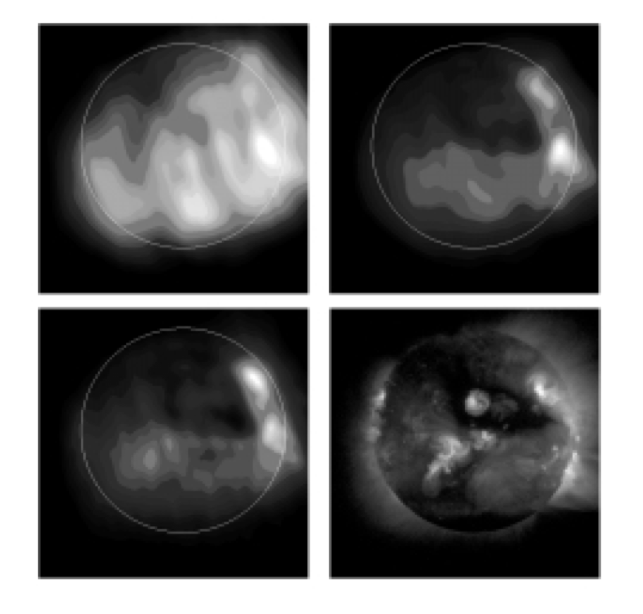
\includegraphics[scale=0.6, trim=0cm 1cm 0cm 1cm]{images/low_freq_obs}
\caption[Comparison of soft X-ray and low frequency radio observations of the corona]{Low frequency observations of the solar atmosphere. Nan\,{c}ay Radioheliograph (NRH) 164MHz (top left), 327\,MHz (upper right), and 410\,MHz bottom left. Yohkoh Soft X-ray Telescope (SXT) image for comparison. Note the coronal holes in the SXT image is also in the 164 MHz image of NRH. The active regions are also bright at 327\,MHz and 410\,MHz \citep{lantos1999}}
\label{fig:lowfreq}
\end{center}
\end{figure}

The quiet corona at metric wavelengths is primarily an emitter of thermal Bremsstrahlung i.e., thermal electrons accelerating in the Coloumb electric fields of protons. The height at which metric radiation escapes from the corona depends on the Bremsstrahlung absorption process, known as free-free opacity and given by
\begin{equation}
\kappa_{ff} \sim \frac{n^2}{\nu^2T^{3/2}} 
\end{equation}
where $n$ is the electron number density, $\nu$ is the frequency of electromagnetic radiation, and $T$ is the temperature. Qualitatively, for a given frequency the density must drop below a certain value for the radiation to become optically thin and escape the solar atmosphere. In the radio band, even the highest frequency (microwaves) do not escape until densities drop to chromospheric values. Hence a microwave image of the sun will provide a direct observation of light escaping from the chromosphere. Reducing the frequency further still to the $10^{8}$\,Hz (metric wavelengths), the density must drop to coronal values before the free-free opacity is low enough for radiation to be optically thin. Hence, metric wavelength radiation escapes the solar atmosphere only in the outer corona. For example 150\,MHz imaging of the solar atmosphere may image an optically thick atmosphere out to a height of $\sim$0.5$\,R_{\odot}$ above the photosphere. The existence of an optically thick atmosphere at these wavelengths allows a direct probing of coronal temperatures at these heights. Using the solution to the radiative transfer equation
\begin{equation}
T_B = T_0e^{-\tau_{\nu}} + T_e(1-e^{-\tau_{\nu}})
\label{eq:rad_trans}
\end{equation}
where $T_B$ is the observed brightness temperature, $T_0$ is the background source brightness temperature, and $T_e$ is the electron temperature of a cloud of plasma between observer and source\footnote{Note that radio observations often use brightness and electron temperatures in place of specific intensity and the source function because radio observations are often calibrated via a load of known temperature}, we can separate this equation into two regimes. Firstly,
in the optically thick regime $\tau_{\nu}>>1$ equation~\ref{eq:rad_trans} reduces to $T_B = T_e$, indicating that the brightness temperature is a direct measure of the electron temperature in solar atmospheric plasma. Secondly, in the optically thin regime $\tau_{\nu}<<1$, equation~\ref{eq:rad_trans} reduces to 
\begin{equation}
T_B = T_0(1-\tau_{\tau}) + T_e\tau_{\nu}
\end{equation}
Considering the case of no background source we see that for the optically thin regime $T_B = T_e\tau_{\nu}$ i.e., the brightness temperature is not a direct measure of the electron temperature, but is reduced by a factor of $\tau_{\nu}$. 
\begin{figure}[t!]
\begin{center}
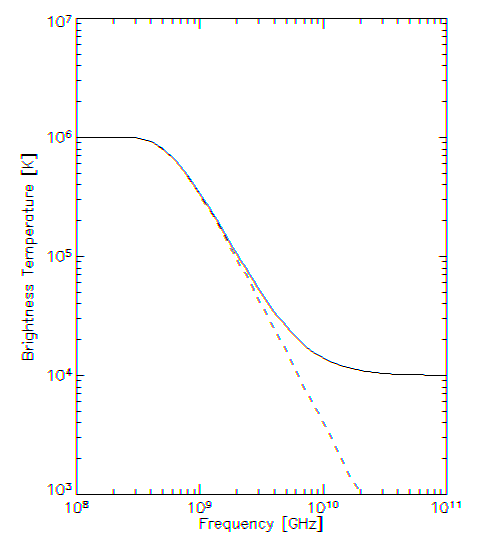
\includegraphics[scale=0.5]{spectral_turnover.png}
\caption[Comparison of soft X-ray and low frequency radio observations of the corona]{Thermal Bremsstrahlung brightness temperature spectrum for an iso-thermal solar corona at $10^6$\,K, plus a 10,000 K chromosphere. The dashed line shows 
the result without a chromosphere. Spectral turnover occurs at approximately 10\,GHz when the coronal plasma becomes optically thin. The plateauing of the solid line beyond $10^{10}$\,Hz is due to observation of an optically thick 10,000\,K chromosphere at these frequencies.}
\label{fig:spectral_turnover}
\end{center}
\end{figure}
Hence, radiation from an optically thick plasma provides a direct probe of the electron temperature in the corona, while radiation from an optically thin plasma provides a measure of the same temperature but diminished by the optical depth. For example, observation of the brightness temperature at a height in the corona where 100\,MHz is optically thick will give $T_b\sim10^6$\,K, provided the radiation field is in thermal equilibrium with a Maxwell-Boltzmann distribution of electrons with $T_e\sim10^6$\,K. At the same height in the corona 10\,GHz will be optically thin so the observed brightness temperature will drop to $\sim10^{5}$\,K. This is why the observed intensity of emission follows electron temperatures up to a frequency of $\sim$10\,GHz, after which there is a `spectral turnover' and the intensity starts to drop rapidly due to the plasma becoming increasingly optically thin (Figure~\ref{fig:spectral_turnover}).

%It is also possible to observe non-thermal sources, in which case the observed brightness temperature is related to the average energy of the emitting particles $<E>=kT_{eff}$, where $k$ is Boltzmann's constant. In such a case, the brightness temperatures may be in excess of $10^{9}$\,K, although the brightness 

%If the electrons are in thermodynamic equilibrium with the radiation field then $T_e$ is simply the temperature of the plasma $T$, given by the Maxwell-Boltzmann distribution, meaning a measure of brightness temperature allows a direct probing of the coronas thermal properties at this height. For example, a measure of brightness temperature at 100\,MHz will given $T_b\sim10^6$\,K. However, beyond 1\,GHz the corona becomes optically thin and brightness temperature then drops to $\sim10^{5}$\,K. It is also possible to observe non-thermal source, which is related to the average energy of the emitting particles $<E>=kT_{eff}$, where $k$ is Boltzmann's constant. In such a case, the brightness temperatures may be in excess of $10^{9}$\,K

%It is also possible to observe non-thermal source in the solar atmosphere, especially during times of high activity. In the case of non-thermal radiation, $T_e$ is replaced by $T_{eff}$, the effective temperature, which is related to the average energy of the emitting particles $<E>=kT_{eff}$, where $k$ is Boltzmann's constant. In such a case, the brightness temperatures may be in excess of $10^{9}$\,K. These emissions are usually associated with flaring and eruptive activity and include gyrosynchrotron emission and plasma emission resulting. Since the observation of plasma emission is partly the subject of this thesis, it will be returned to in detail in chapter 2.
%\subsection{Solar Wind}\label{sec:13}

%\begin{itemize}
%\item Parker's solution
%\item Parker Spiral
%\item Fast solar wind, Alfv\'{e}n wave driver
%\item Mass loss rates (later compare CME mass loss)
%\end{itemize}



\section{Coronal Mass Ejections}\label{sec:2}

%The solar corona is home to a variety of dynamic and highly energetic activity, the cause of which is the build-up and release of magnetic energy. This energy release results in the acceleration of charged particles, emission of electromagnetic radiation across the entire spectrum, the heating of plasma, the ejection of large scale eruptions and the driving of plasma shocks through the corona and heliosphere. Large scale eruptions of plasma and the driving of shocks are the subject of this thesis, the following provides an observational overview and open questions concerning these phenomena.

The solar corona is home to a variety of dynamic and highly energetic activity, the cause of which is the build-up and release of magnetic energy. Of all the activity taking place in the corona, the most spectacular manifestation of energy release is the coronal mass ejection (CME). A modern understanding of corona mass ejectionss tells us that they are large-scale eruptions of plasma and magnetic field that propagate from the low solar corona into interplanetary space. They have speeds in the range $10-2500$\,km$\cdot$s$^{-1}$ \citep{gopal2004}, masses of $10^{13}-10^{16}$\,g, and kinetic energies of $10^{22} - 10^{25}$\,J \citep{vour2010}, making them the most energetic explosive events in the solar system and a major cause of adverse space weather in the near-Earth environment. The following provides an observational overview and open questions concerning the general properties of CMEs, including their morphology, kinematics, and dynamics, as well as their ability to drive shocks, accelerate particles, and produce a variety of radio bursts.

\subsection{A Brief History}\label{sec:20}

The largest flare ever to have been recorded occurred on September 1st 1859, observed by the astronomer Richard Carrington \citep{carrington1859}. Approximately 17 hours after Carrington recorded the event, a powerful geomagnetic storm began at Earth, producing brilliant aurora and damaging telegraph systems on both sides of the Atlantic ocean. The event aroused much speculation on a causal link between the phenomena Carrrington observed on the Sun and the magnetic activity recorded throughout the Earth \citep{balfour1861}. It was not until 1919 that a theory was put forward to suggest plasma transients emitted from the Sun may impact the Earth and cause geomagnetic activity and the aurora \citet{lindemann1919}, a process later elaborated upon by \citet{chapman1930}. Up until 1940s, the only evidence confirming the plasma transient hypothesis was the correlation between solar and geomagnetic activity. However, following the development of radio receiver technology during World War Two, much interest was given to solar radio bursts and their indication that disturbances travel away from the Sun at speeds of up to 500\,km\,s$^{-1}$\citep{wild1958}. Further evidence came from the fields of cosmic rays studies, when it was suggested the ground level detections of particles at Earth such as those reported by \citep{forbush1946} may be related to a acceleration of particles by a shock moving through the solar atmosphere \citep{wild1963}. Eventually this activity was summarised by \citet{gold1962}, who hypothesised the expulsion of magnetized plasma from the solar atmosphere and the driving of a shock by this expulsion tha accelerates particles into interplanetary space. 

Gold's paper marked over 100 years of indirect evidence for the expulsion of plasma transients from the surface of the Sun toward Earth. However, it was not until December 14th, 1971 (112 years after the Carrington event) that the first direct images of one of these plasma expulsions was made with the coronagraph on board the 7th Orbiting Solar Observatory (OSO-7) satellite \citep{tousey1971}. This marked the beginning of white-light CME studies as we know them today, and it was followed by a number of other instruments, including Skylab \citep{macqueen1980}, P78-1 \citep{sheeley1980}, and the Solar Maximum Mission (SMM) \citep{hundhausen1999}, which provided corongraph observations up until 1989. The modern era of CME observations began 1995 with the launch of the Solar and Heliospheric Observatory \citep[\emph{SOHO};][]{dom95} and its more sophisticated suite of instruments, including the Large Angle Spectrometric Coronagraphs (LASCO). In 2006 LASCO was joined by the COR coronagraphs onboard the Solar Terrestrial Relations Observatory \citep[\emph{STEREO};][]{kai08} and together they provide observations of CMEs from the low solar atmosphere into interplanetary distances. The past 40 years of coronagraph operations in space have yielded observations of tens of thousands of CMEs, allowing a direct determination of their physical properties and a confirmation of what was first postulated by Carrington and others over 150 years ago.

\subsection{Morphology and Kinematics} 

%------------------------------- Appearance, Size, Width -------------------------------------%

CMEs are most often observed using a coronagraph, an instrument that creates an artificial eclipse of the bright solar disk so the much fainter corona can be imaged (this instrument is described in detail in Chapter 3). Figure~\ref{fig:lasco_c3} shows the typical appearance of a CME in white light coronagraph images, having a three-part structure of bright front, followed by a darker cavity, and a bright core \citep{illing1985}. Although this CME is regarded as \textquoteleft typical' in appearance, many CMEs do not have all of these features and some appear to have more complex morphological structures \citep{pick2006}, with only around 30\% of all CMEs exhibiting the three part structure \citep{webbHu1987}. 
\begin{figure}[t!]
\begin{center}
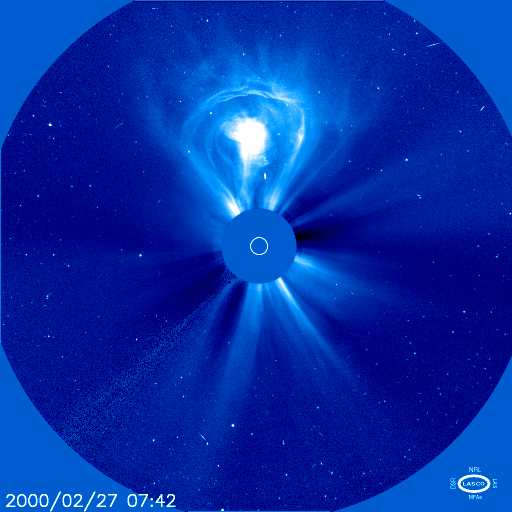
\includegraphics[scale=0.45]{images/lasco_c3}
\caption[LASCO C3 image of a CME]{Large Angle Spectrometric Coronagraph (LASCO) C3 coronagraph image of a \textquoteleft typical' CME, showing  a bright front surrounding a dark cavity, with a bright core at the centre. The central disk is the occulter of the coronagraph, blocking out the bright light of the solar disk, so the much fainter corona may be imaged. The white circle represents the solar disk.}
\label{fig:lasco_c3}
\end{center}
\end{figure}
The varied nature of their appearance and morphology can usually be attributed to projection effects \citep{burk2004} i.e., the CME is a 3-D object projected onto a 2-D image, hence its appearance depends on its orientation in the corona. With this in mind, a `plane-of-sky' or limb CME (one that erupts on the solar limb and propagates at right angles to the observer-sun line), offer the best measure of their properties i.e., the measured widths, appearance, speeds etc. do not suffer projection effects. Limb CMEs have a typical angular extent of approximately $50^{\circ}$ \citep{burk2004}, and any CME that has width much greater than this ($>120^{\circ}$) is generally regarded as a `partial halo' CME \citep{yashiro2004}. Halos or partial halos are CMEs that propagate toward the observer and hence appear to have a very wide angular extent (full halos can appear to have a $360^{\circ}$ width), due to projection effects. However, statistics to characterize a typical CME size often only consider large `classical' CMEs i.e., those ejections that generally appear typical are included, but the much smaller and very narrow ejections (widths $<15^{\circ}$) are excluded. The exclusion of small ejections means that typical CME size is normally distributed about $40-50^{\circ}$. However, some studies account for these small ejections and simply consider any mass ejection, no matter how small, as a CME \citep{robb2009}. Inclusion of the very small ejections has found the possibility of scale invariance in CME size, with the distribution being described by a power law. \citet{robb2009} has suggested that their is no \textquoteleft typical' CME size.


%------------------------------- 3D Studies -------------------------------------%

The majority of CME observations rely on a 2-D projection onto the plane of sky, thereby  disguising their true three-dimensional shape and geometry. Despite the majority of CME studies being constrained to 2-D measurements, there have been various studies whereby the full 3D extent of the CME bubble has been reconstructed. \citep{moran2004} used polarimetry measurements from the LASCO coronagraphs to reconstruct the three dimensional extent of the CME using Thomson scattering theory (the degree of polarization of white-light depends on the location of the scattering agent in 3-D space). When the STEREO spacecraft were launched in 2006 a number of stereoscopy techniques were developed that use geometric localization, whereby the CME is constrained to be within a polygon constructed from lines of sight from the two STEREO spacecraft \citep{dekon2009, byrne2010}. Other techniques use a pre-assumed 3D construct that is oriented so that a 2-D projection of the construct matches the observed 2-D image of the CME. This technique is known as forward-modeling and usually employs a graduated cylindrical shell or 'croissant' model as the pre-assumed shape of the CME \citep{thern2006}. Finally, other techniques employ a number of the above techniques simultaneously or for comparison of which preforms best \citep{mierla2009}. Although each of these studies have derived much more accurate CME properties such as size, shape, and kinematics that do not suffer projection effects, this has only been performed for a handful of cases. Unfortunately, typical CME statistics must suffer the unavoidable uncertainties of 2-D coronagraph observations. Perhaps the most egregious errors brought about by lack of three dimensional CME measurements are CME mass calculations, the subject of Chapter 4 of this thesis.

Despite the projection effects, reasonable CME kinematic properties may be derived if the CME is located in the limb or the general direction of propagation is accounted for. A number of CME catalogues exist that have tracked and analysed thousands of events, most throughout the SOHO mission. Measured properties include, CME launch latitude, speed, acceleration, and, where possible, masses and energies. The latitudinal distribution of CME launches depends on the solar cycle, with the majority of CMEs erupting close the equator at solar minimum, and generally at all latitudes occurring during solar maximum \citep{yashiro2004}.

%------------------------------- Velocity, Acceleration -------------------------------------%

The amount of CMEs observed during the SOHO era (which continues today) has allowed many statistical studies of CME speeds and accelerations. CME speeds can range from 20 to 2500\,km\,s$^{-1}$ \citep{gopal2004}, however average CME speed tends to be on the order of 480\,km\,s$^{-1}$ \citep{yurch2005, webb2012}\footnote{Statistical studies from the era of Solar Maximum Mission and Solwind have found similar average speeds \citep{burk2004}}. The yearly average of CME speeds tends to change with the solar cycle, with an average of 280\,km\,s$^{-1}$ at solar minimum (1996), followed by a year on year increase in speed until an average of 520\,km\,s$^{-1}$ is reached even after solar maximum (2002) i.e., for solar cycle 23 the CME speed continued to rise even during the declining phase of the solar activity cycle \citep{yashiro2004}. There has been some debate surrounding the possibility of a bimodal distribution of CME speeds, generally considered a distinction between fast and slow CMEs. Slow CMEs with a speed of $400-600$\,km\,s$^{-1}$ and gradual acceleration are usually associated with prominence lift-off, while fast CMEs with speeds in excess of 700\,km\,s$^{-1}$, no acceleration (or small deceleration), and are usually associated with flaring active regions \citep{shee1999, gopal2004, moon2000}. Other statistical studies have suggested that there is no such distinction between the speeds of filament-associated and flare-associated CMEs \citep{vrsna2005, yurch2005}, with all CME having a more continuous distribution in speeds rather than a bimodal one (Figure~\ref{fig:yurch2005}). 
\begin{figure}[!t]
\begin{center}
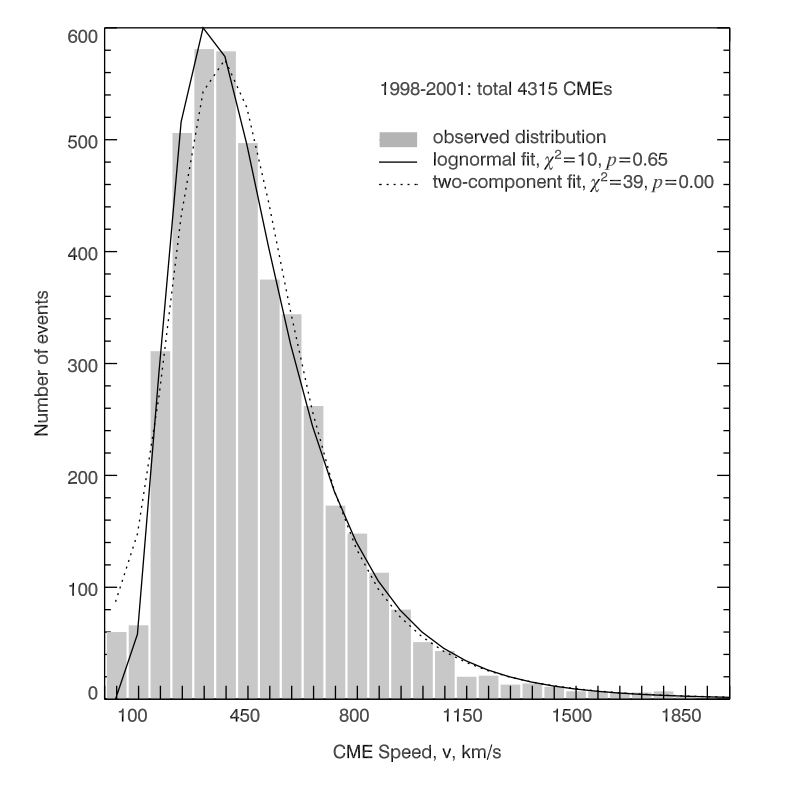
\includegraphics[scale=0.4, trim=0cm 1cm 0cm 1cm]{images/cme_speed_histo}
\caption[Distribution of CME speeds]{Distribution of speeds of 4315 CMEs observed by SOHO LASCO. The bin widths are 70\,km\,s$^{-1}$. The solid line represents a single lognormal fit to the observed data, while the dashed line is the sum of a Gaussian and a lognormal fit. \citep{yurch2005} }
\label{fig:yurch2005}
\end{center}
\end{figure}
\begin{figure}[t!]
\begin{center}
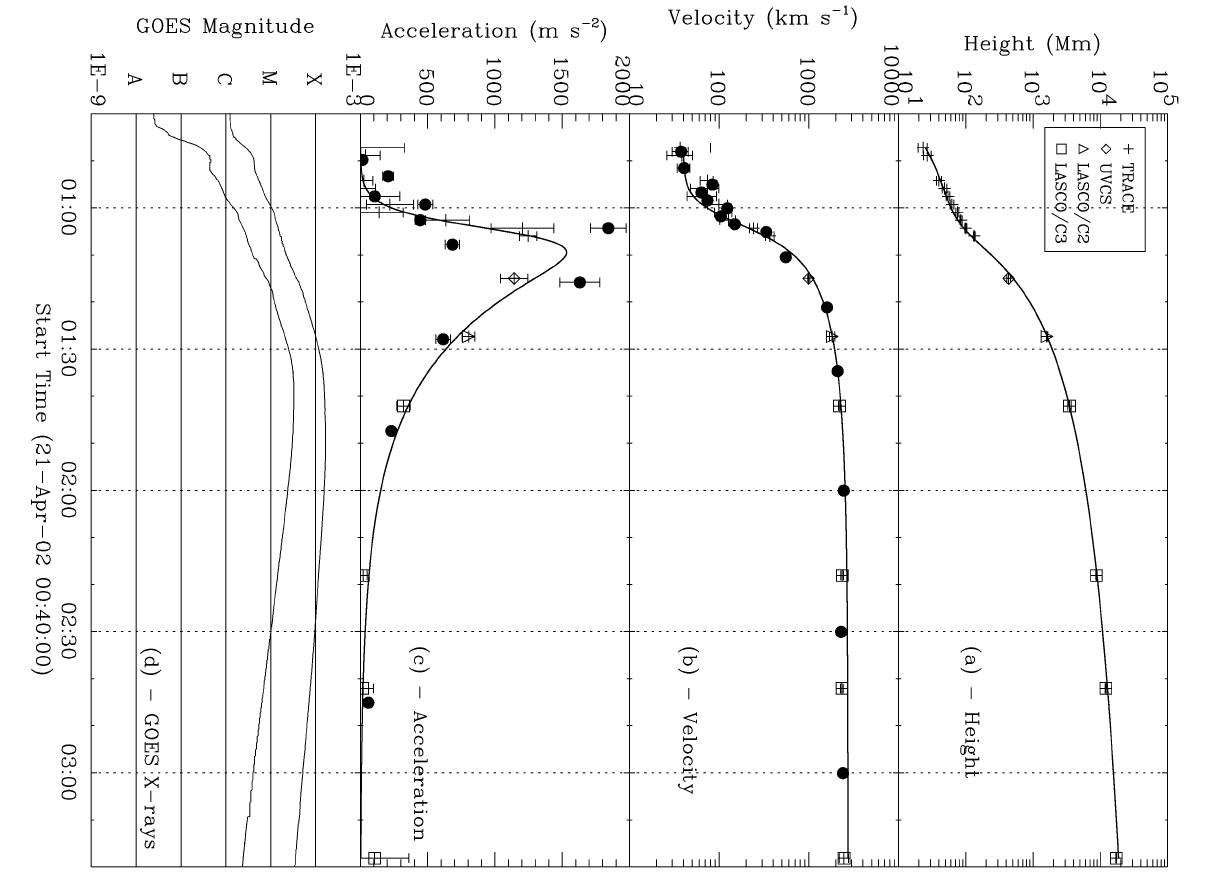
\includegraphics[scale=0.35, angle=90, trim=1cm 0cm 2cm 2cm]{images/gall_kins2003}
\caption[CME height, speed, and acceleration as function of time]{CME kinematics derived from TRACE, UVCS and the SOHO LASCO coronagraphs. The height time data is used to derive velocity and acceleration. The CME shows a peak in acceleration early in its propagation, this peak is coincident with the flare impulsive phase (indicated by the GOES) light curves in the bottom plot \citet{gallagher03}}
\label{fig:gall2003}
\end{center}
\end{figure}
This more continuous distribution is also reflected in statistical studies of low coronal CME acceleration magnitudes and timescales. Although typical CME accelerations in the later phases of propagation tend to be centered around zero with a narrow variation of $\pm30$\,m\,s$^{-2}$, CME accelerations in the very early phases of eruption can be considerably larger. \citet{gallagher03} used TRACE and LASCO data to study the development of the kinematics of a CME from its very early impulsive phase with peak acceleration of $1500$\,m\,s$^{-2}$ to a more gradual phase of zero acceleration (Fig.~\ref{fig:gall2003}). 

A larger statistical study by \citep{zhang2006} using all three LASCO coronagraphs covering $1.1-30\,R_{\odot}$ found accelerations in the range of $2.8-4464$\,m\,s$^{-2}$ with an average of 330\,m\,s$^{-2}$, with the acceleration timescales ranging $6-1200$\,minutes (average of 180 minutes). An interesting outcome of this study was the discovery that the magnitude of acceleration appears to be inversely proportional to the duration of acceleration (Fig.~\ref{fig:acell_duration}), following the relationship $a=1\times10^4t^{-1}$.

\begin{figure}[t!]
\begin{center}
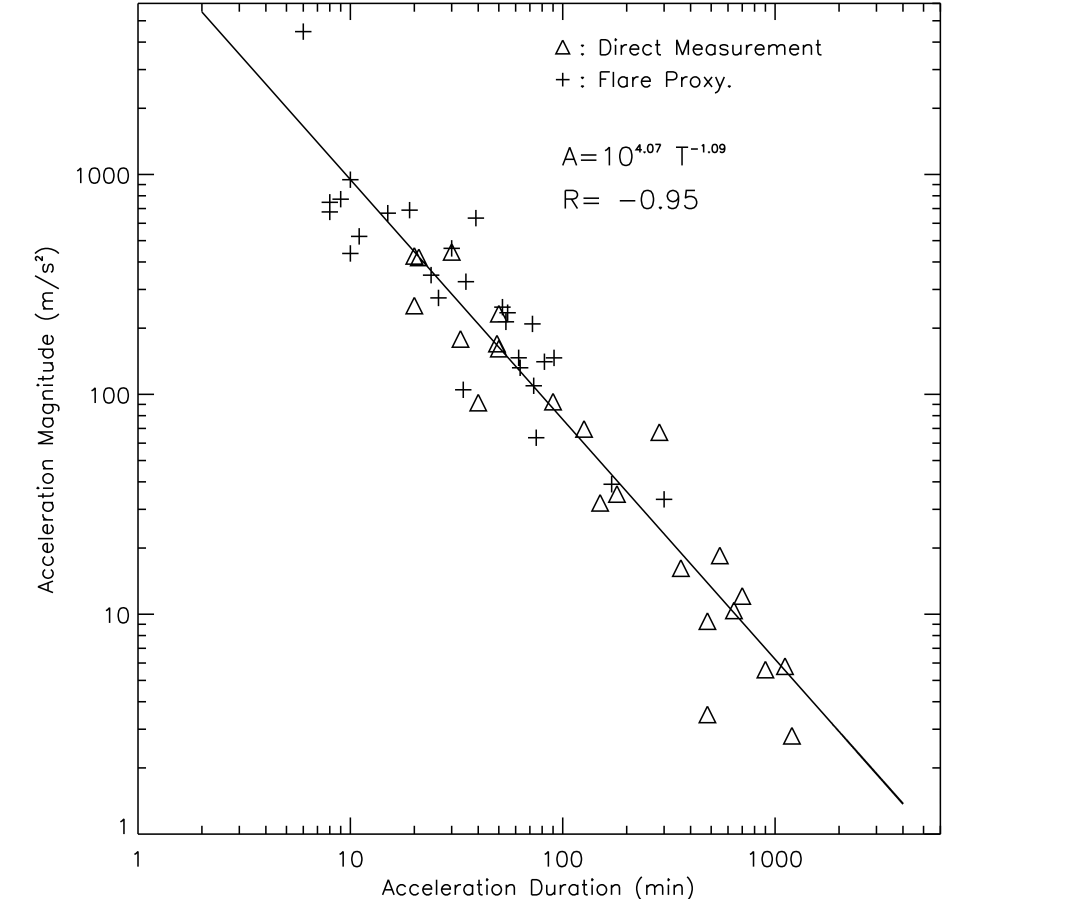
\includegraphics[scale=0.25]{images/accel_zhang2006}
\caption[CME acceleration as a function of acceleration duration]{Acceleration of CMEs vs the duration of the acceleration. The data show an inverse proportionality i.e., shorter acceleration durations leads to larger magnitudes of acceleration \citep{zhang2006}}
\label{fig:acell_duration}
\end{center}
\end{figure}
Unfortunately the innermost coronagraph of LASCO (C1) failed in 1998, making early phase studies of CMEs difficult. Due to the failure of C1, the only observational method to determine the early phase eruption kinematics has been with EUV imaging.
Such statistical studies also show similar results of initial impulsive phase accelerations of $\sim10-4000$\,m\,s$^{-2}$, followed by a residual phase of near zero acceleration \citep{vrsnak2007, temmer2010}. A large acceleration during the impulsive phase followed by a smaller (or zero) acceleration is recognized as being part of three distinct phases of eruption that closely tie the CME process to the flaring process, Fig.~\ref{fig:zhang2001}. \citet{zhang2001, zhang2004} reported that CMEs show a very slow rise phase of coronal loops with a speed of $10-100$\,km\,s$^{-1}$ over tens of minutes. This is followed by a phase of rapid acceleration which is accompanied by a simultaneous rise in soft x-ray (SXR) emission, as seen in a GOES light curve. After the flare, and during the decline of SXRs, the CME shows a near constant velocity with very little acceleration. The simultaneous rise of SXR emission at the time of maximum CME acceleration is taken to be an effect of the CME and the flare both being manifestations of the same energy release in the corona.

\begin{figure}[t!]
\begin{center}
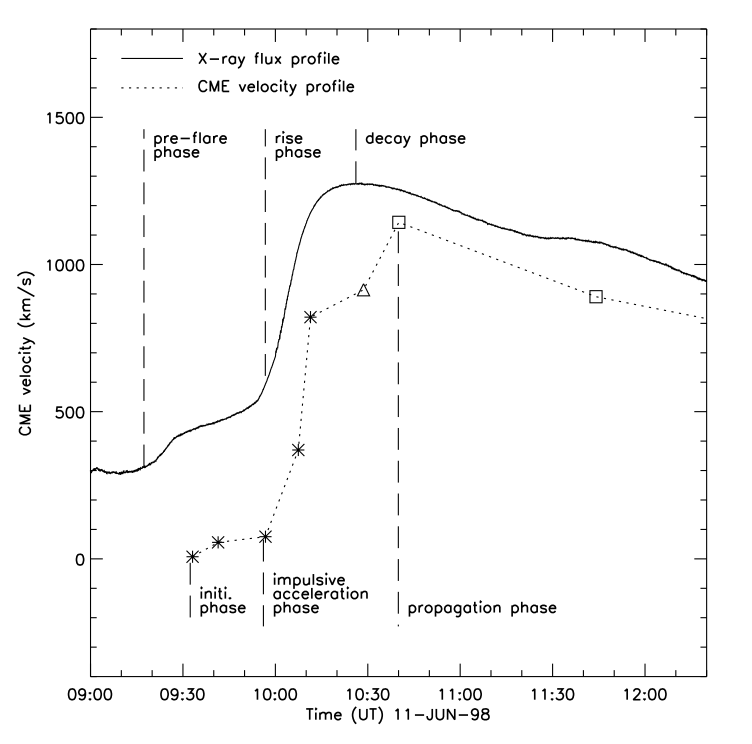
\includegraphics[scale=0.4, trim =0cm 1cm 0cm 1cm]{images/zhang2001}
\caption[CME speed profile along side flare X-ray light curve]{Correspondence between CME velocity profile and soft x-ray light curve from GOES. The two profiles follow each other closely showing that CME acceleration occurs during the flare rise phase. this is taken to be an effect of the CME and the flare both being manifestations of the same reconnection process \citet{zhang2001}.}
\label{fig:zhang2001}
\end{center}
\end{figure}

\subsection{Masses and Dynamics}
%------------------------------- Masses -------------------------------------%

As mentioned above, many properties of CMEs derived from two-dimensional coronagraph images suffer large uncertainties due to lack of knowledge about the true three-dimensional shape of the object. Despite this, much work has been done on CME kinematics and the general velocity and acceleration evolution is now well known. However, much less work has been done on the observational properties of CME dynamics e.g., calculating their mass, mechanical energies and forces. 

Some of the first measurement of CME mass using scattering theory were carried out by \citet{munro1979} and \citet{poland1981} using space-based  white light coronagraphs on board \emph{SkyLab} and U.S. military satellite\,\emph{P78-1}.  Both the early studies and later statistical investigations determined that the majority of CMEs have masses in the range of 10$^{13}$--10$^{16}$\,g, \citep{vourlidas02, vour2010}. However, due to only a single viewpoint of observation, the longitudinal angle at which the CME propagates outwards was largely unknown in these studies and it is generally assumed that the CME propagates perpendicular to the observers line-of-sight (LOS). There is also the added assumption that all CME mass lies in the two-dimensional plane-of-sky (POS). Such assumptions can lead to a mass underestimation of up to 50\% or more \citep{vou00}. More recent studies have employed the two viewpoint capabilities of the \emph{STEREO} mission to determine the mass of numerous CMEs with much less uncertainty \citep{cola09}. These few studies remain the only investigation into CME masses and the field has been largely overlooked due to the huge uncertainties involved in mass calculations (described in Chapter 4).

While the majority of mass estimates have come from white-light observations of CMEs, other wavelengths offer an independent measure of CME mass estimates, usually via a different technique which pertains to the wavelength being observed. The eruption of a CME as seen by EUV imaging of the corona often shows a region of diminished intensity around the active region from which the eruption took place. This is known as an EUV dimming, and is indicative of a mass evacuation i.e., the CME carries mass away when it erupts leaving behind a deficiency in emitting material.  
%If this intensity deficiency is compared to the pre-event intensity, and the volume of the emitting region is estimated, then the mass in the dimming region may be derived. This is done for multiple filters in EUV imaging such as EUVI 171, 195, 284\,\AA. From this a mass deficiency distribution across temperature may derived, the integration of which will yield the total mass evacuated from the CME source region \citep{aschw09}. 
\citet{aschw09} calculated the mass from EUV dimming $m_{EUV}$ and compared it to the mass measured in white-light $m_{wl}$ and found a close match of $m_{EUV}/m_{WL}=1.1 -1.3$. Although this technique provides a rare measure of the CME mass in the very early stages of eruption, few studies have used this in conjunction with the white-light measurements.

Perhaps the only measurement of CME mass via direct low frequency radio imaging was performed by \citet{gopalswamy1992}. An event observed on 6 February 1986 by Clarke Lake multifrequency radioheliograph showed an erupting structure at 73\,MHz. On the assumption that the emission mechanism was thermal bremsstrahlung in an optically thin environment, an estimate of the emitting mass was calculated and shown to be $2.7\times10^{15}$\,g, similar to what is generally reported in white-light studies. Despite the interesting techniques afforded by radio observations, they are still not as popular as the white-light measurements of mass, due to the rarity of actually observing a CME at long wavelengths.


%A rare measure CME mass through low frequency radio measurements was presented by \citet{gopalswamy1992}. Very few CMEs have been observed at metric wavelengths, but an event on 16 February 1986 observed by Clarke Lake multifrequency radioheliograph clearly showed an erupting structure at 73\,MHz. On the assumption that the emission mechanism was thermal bremsstrahlung in an optically thin environment, an estimate of the emitting mass was calculated and shown to be $2.7\times10^{15}$\,g, similar to what is generally reported in white-light studies. Despite the interesting techniques afforded by EUV and radio observations, they are still not as popular as the white-light measurements of mass. This is in part due to the ambiguity of identifying CMEs at ultraviolet or radio. In EUV the CME is part of a complex and evolving low corona and it is generally difficult to distiguish and erupting structure from evolving active region. As for radio, only part of the CME may be emitting, not to mention the rarity of CME observations at low frequencies.
%------------------------------- Energies -------------------------------------%
\begin{figure}[t!]
\begin{center}
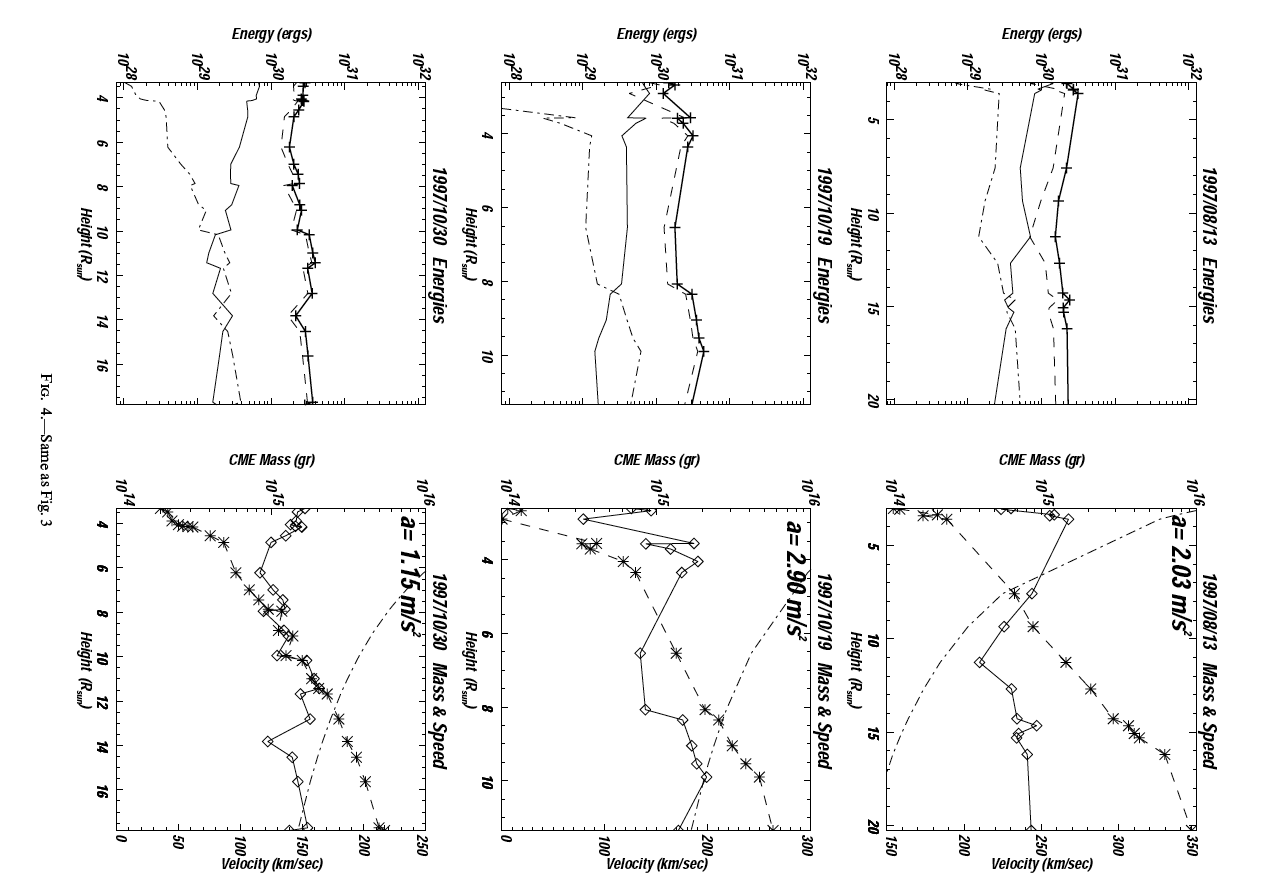
\includegraphics[scale=0.4, angle=90, trim=1cm 0cm 2cm 2cm]{images/cme_energies}
\caption[CME energies and masses as a function of height]{Coronal mass ejection energies and masses as a function of height for three different events.
Left coulumn shows the CME kinetic (solid), potential (dashed), magnetic (dot-dashed), and total energy as a function
height. In each of the plots, kinetic an potential energy increases at the expense of decreasing magnetic energy. The total energy 
remains quite constant, showing that there is no external driver of the system. Right column, CME mass (solid), center of mass speed (dashed), and escape velocity (dot-dash) as a function of height \citep{vou00}}
\label{fig:cme_energies}
\end{center} 
\end{figure}
Given the relative ease with which CME positions and velocities may be determined, there are only a small number of studies which combine these kinematic properties with the mass estimates in an effort to derive CME mechanical energy budgets. The first study to address the issue in the SOHO era attempted to quantified the magnitude of the kinetic and gravitational potential energy and compared this to a proxy for the magnetic energy from in-situ measurements of magnetic clouds \citep{vou00}. Out of the 11 CMEs that were studies, it was found that the CMEs mechanical energy increases at the expense of magnetic energy, Figure~\ref{fig:cme_energies}. The forms of these energies are given by
\begin{eqnarray}
E_{kinetic} & = & \frac{1}{2}\sum m_i v_{cm}^2 \\
E_{potenial} & = & \sum \int_{R_{\odot}}^{R} \frac{GM_{\odot}m_i}{r^2_i}\\
E_{magnetic} & = & \frac{1}{8\pi}\int B^2 dV
\end{eqnarray}
where $m_i$ and $r_i$ are the CME mass element and distance from Sun center, respectively, $v_{cm}$ is the center of mass velocity, $M_{\odot}$ and $R_{\odot}$ are solar mass and radius, respectively, $B$ is the CME magnetic field, and V is its volume. The summation is carried out of each CME mass elements i.e., each image pixel that includes the CME. The total energy of the CME (kinetic + potential + magnetic, usually on the order of $10^{30}$\,erg) remains constant, indicating that there is no external driver of the CME between $3-30\,R_{\odot}$. Hence, CMEs much achieve escape velocity to exit the Sun's gravitational potential well, which they do so between $8-10\,R_{\odot}$. For slow to average speed events, the potential energy dominates the kinetic energy by an order of magnitude, the opposite is found for faster events. 

A much larger statistical estimate of CME mechanical energy distribution was performed by \citep{vour2010} for 7668 CMEs observed by LASCO from 22 January 1996 to 31 July 2009 (Figure~\ref{fig:energy_dist}). This is the most comprehensive CME mechanical energy statistics study to date and shows that both kinetic energy and total mechanical energy are normally distributed about $2.3\times10^{29}$\,erg and $9.0\times10^{29}$\,erg, again showing that potential energy (mechanical - kinetic) is dominant over kinetic energy on avarege.
\begin{figure}[h!]
\begin{center}
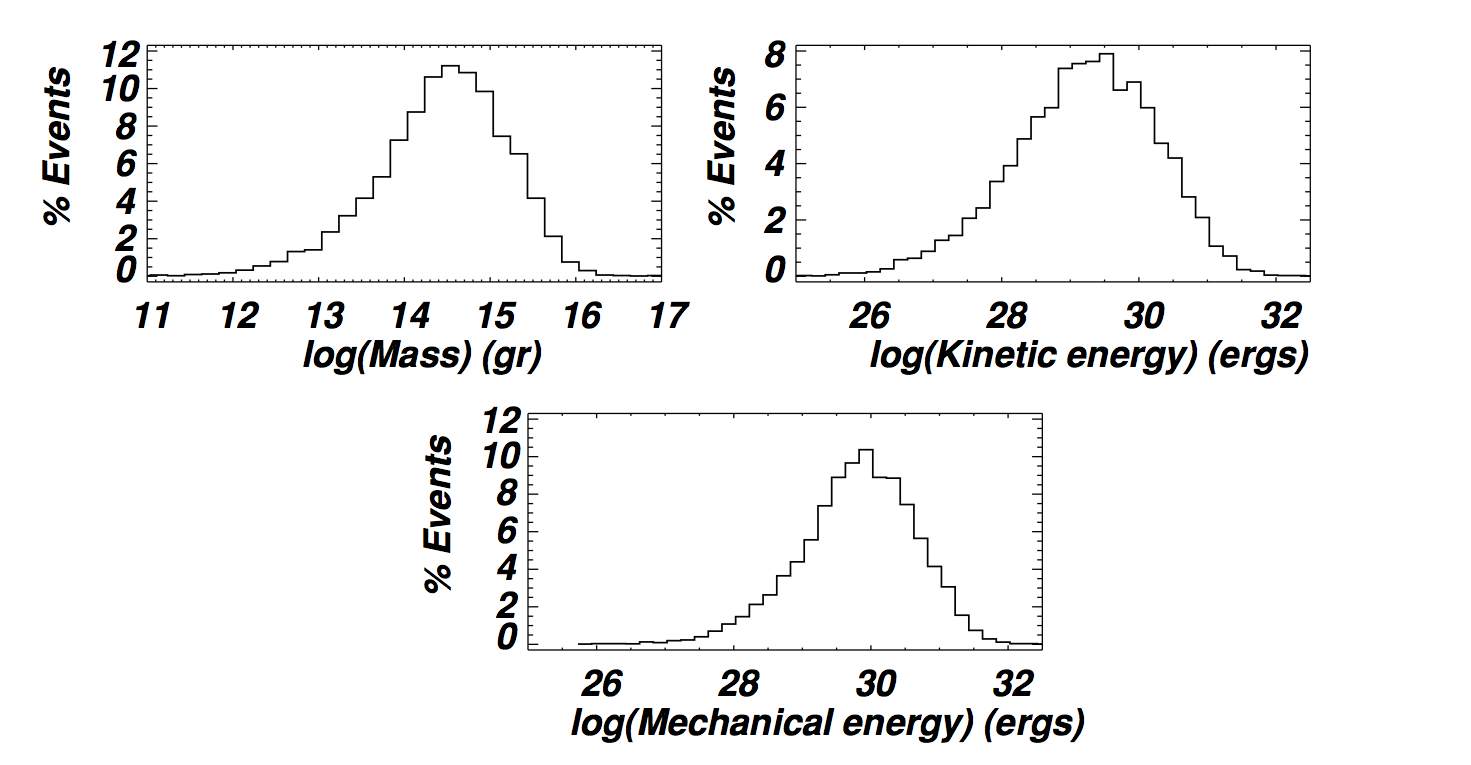
\includegraphics[trim = 1cm 0cm 0cm 3cm, scale=0.3]{images/energy_dist}
\caption[Distribution of CME masses, kinetic and total mechanical energies]{Distribution of CME masses, kinetic and total mechanical energies for 7668 CMEs observed by the LASCO
coronagraphs between 1996 January 22 to 2009 July 31. The peak in kinetic energy is $2.3\times10^{29}$\,erg, while total mechanical energy is $9.0\times10^{29}$\,erg \citep{vour2010}}
\label{fig:energy_dist}
\end{center}
\end{figure}

\citep{subram2007} investigated the energetic properties of 39 CMEs in an effort to determine if CMEs in the outer corona ($2-20\,R_{\odot}$) are driven by momentum coupling to the solar wind or if internal magnetic energy is a viable source of driving power. They found that in 69\% of the cases the mechanical energy of the CME increased linearly with time, an effect that suggests CMEs are driven by the gradual release of some form of energy. The estimated total power delivered to the CME to increase its mechanical energy was 1.6\,erg\,hr$^{-1}$, which is far below the upper limit to the total power dissipated by the magnetic field in the CME (14.4\,erg\,hr$^{-1}$). This is taken to be a suggestion that the CMEs magnetic field is the ultimate source of energy that drives its propagation, even out to large heliocentric distances distances. However the magnetic field estimates in this study are tenuous at best, and any magnetic power estimated derived from them should be treated with caution. \citet{lewis2002} found that the solar wind may be a significant contributor to CME driving power, accounting for some proportion of an average $2.2\times10^6$\,W\,kg$^{-1}$ required to drive the CME, however the authors do not mention quantitatively the possible driving power of the wind, merely calling the wind an \textquoteleft infinite energy reservoir'. Hence it is difficult to affirm the possibility of their assertions.
s
%------------------------------- Forces -------------------------------------%

Perhaps one of the only studies to make an observational estimate of the forces acting on CMEs is \citet{vrs06}, although this study made use of kinematics to infer the dominant forces at play during CME propagation (acceleration is treated  \textquoteleft force-density' or Newtons per kilogram, a pseudo-measurement of force). The early phase eruption characteristics of a H-$\alpha$ spray ejection were analysed to derived the ejection's total acceleration $a$ (Figure~\ref{fig:vrsnak06}). This is recognized as being due to a combination of accelerations due to the Lorentz force $a_L$, gravity $g$, and aerodynamic drag $a_d$, such that $a = a_L -g +a_d$, which results directly form the MHD equation of motion (see Chapter 2, equation~\ref{eqn:mhd_momentum}). Estimates of acceleration due to gravity can be made simply. Expression for drag generally take into account the interaction of the CME with the solar wind whereby drag is given by the difference between the ejecta and wind velocity $|v_{cme} - v_{sw}|$, the area of the ejecta exposed to drag by the wind $A$ and a drag coefficient $C_d$ which usually accounts for the shape of object. The expression may be expressed in quadratic form, $a_d = - \gamma(v_{cme} - v_{sw})|v_{cme} - v_{sw}|$, where $\gamma = C_dA\rho_{sw}/M_{cme}$ \citep{cargill2004}\footnote{Solar wind drag on the CME is discussed further in Chapter 4}. $v_{sw}$ may be given from a model of the solar wind, for example \citet{sheeley1997}. As for the $\gamma$ term,\citet{vrs06} uses empirical scaling laws whereby $\gamma =  23R^{-2.2}$\,km$^{-1}$, where $R$ is the heliocentric distance of the ejecta. When gravity and drag are estimated in this way, a peak Lorentz acceleration is derived to be to be $1400$\,m\,s$^{-2}$. 
\begin{figure}[ts!]
\begin{center}
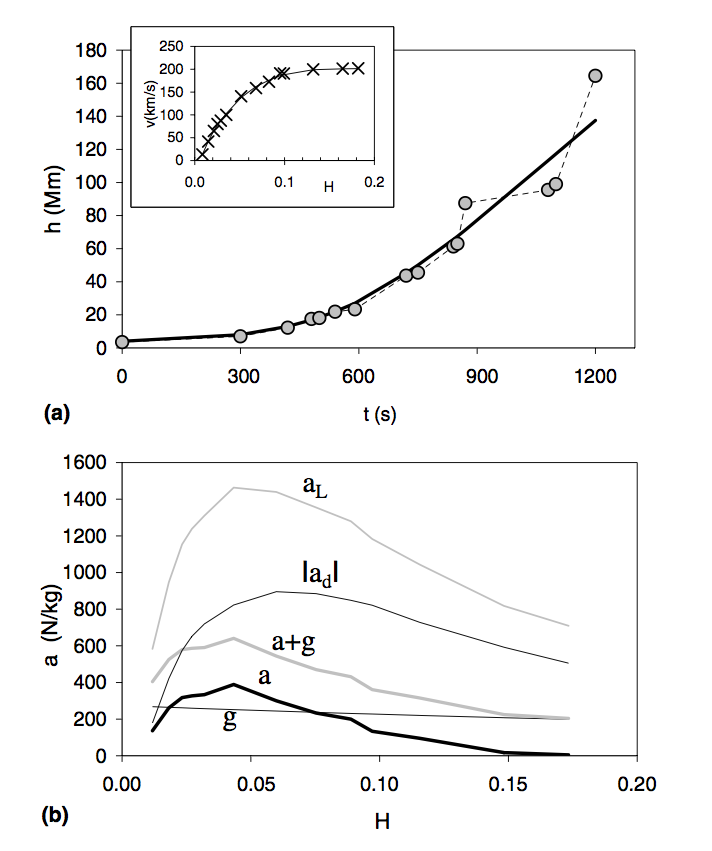
\includegraphics[scale=0.4, trim=0cm 0cm 0cm 2cm]{images/vrsnak_lorentz}
\caption[Acceleration due to all forces acting on CME]{Top: the height-time velocity of a h-alpha spray, with velocity as a function of height inset. Bottom: the acceleration of the spray $a$ as a function of height (derivative of inset in top panel), as well as the acceleration experienced from gravity $a_g$ (also $a+a_g$), drag $|a_d|$, and acceleration due to the Lorentz force $a_L$ \citep{vrs06}}
\label{fig:vrsnak06}
\end{center}
\end{figure}
Taking the particle density of the ejection to be $10^{16}-10^{17}$\,m$^{-3}$ the volume force can then be evaluated as $f_L = 10^{-8}-10^{-7}$\,N\,m$^{-3}$. This is one of the only studies (perhaps the only) in the literature that attempted to derive a size for the Lorentz force, albeit by using an indirect proxy, and also by only looking at a H-$\alpha$ spray. 

Recently \citet{malo10} determined the nature of the drag force acting on CMEs from 3D observations using the STEREO COR1 and COR2 the heliospheric imagers (HIs). It was found that drag on fast CMEs has a quadratic dependence on the velocity difference between the CME and solar wind, while slow CMEs show a linear dependence. This difference may be due to the different nature of the drag force at different at different CME speeds.


A statistical kinematical study was considered by \citep{bein2011}, where a number of parameters were compared, such as max acceleration experienced by the CME, duration of acceleration, and height of maximum acceleration. They find that, as in the \citet{zhang2006} (Fig.~\ref{fig:acell_duration}), the acceleration experienced is inversely proportional to the duration of acceleration, and further, the acceleration experienced and the height of peak acceleration are inversely related. This is taken to be indicative of a compact source size having a more impulsive acceleration, an effect that is consistent with the Lorentz force. Again, the nature of forces acting on CMEs in this case is only inferred from kinematics studies, and not measured directly.

The CME energy budget as compared to the total eruptive energy, including the flare and all by-products. \citet{emslie2004} studied to eruptive energy budgets, taking into account (i) the CME, (ii) the flaring thermal plasma, (iii), the electrons responsible for hard X-rays, (iv) gamma-ray producing ions, and (v) solar energetic particles detected in-situ. Accumulating all of this into an energy budget for the two events found that the CME mechanical energy of $\sim10^{32}$\,erg is the dominant single component of energy consumption, with the flare thermal plasma, non-thermal electrons and ions, and in-situ detected particles, each consuming $\sim10^{31}$\,erg. A similar study was then carried out where the same analysis was applied to 38 eruptive events, which again found that the CME is the dominant consumer of total energy released \citep{emslie2012}
\begin{figure}
\begin{center}
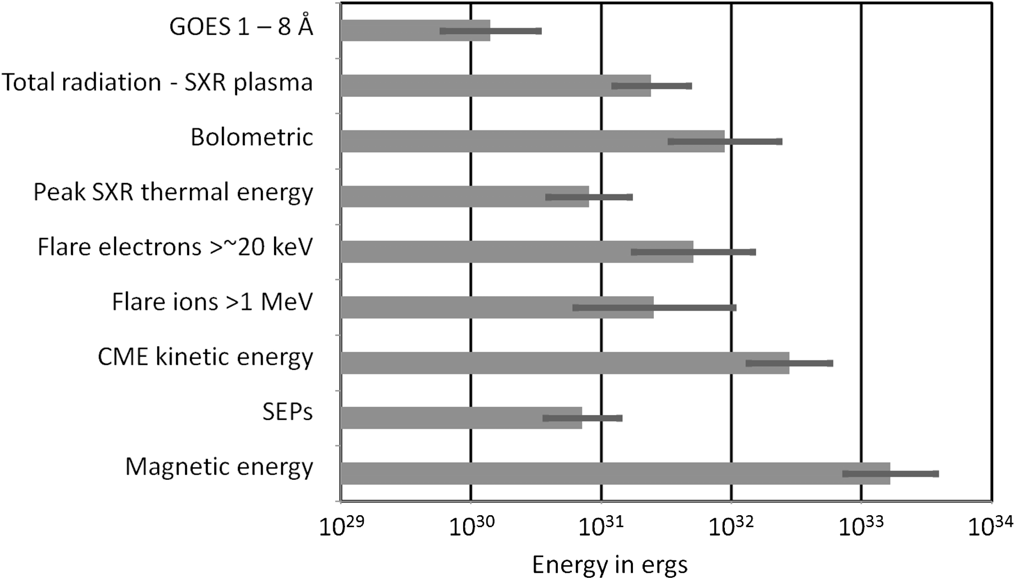
\includegraphics[scale=1.1, trim=1cm 0cm 0cm 0cm]{emslie_energy.png}
\caption{The average energies of the different components of an eruptive event for six events. The CME is the biggest consumer of energy \citep{emslie2012}.}
\label{fig:emslie_energy}
\end{center}
\end{figure}

%The most striking case of this is in the measurement of CME masses, and consequently their mechanical energies and forces. Due to the huge errors involved in 2-D mass calculations, the study has been lacking with only a few papers in the field addressing CME mass and mechanical energy, and fewer still addressing observed CME force estimates. The uncertainties from the method by which mass of a CME is calculated. Thomson scattering theory is employed to derived the number of electron in each image pixel contributing to the total brightness in that pixel. This requires knowledge of where the light scattering agent is in the corona. The lack of knowledge of where the scattering agent is in the third-dimension (along the line of sight) leads to large, and often undefinable uncertainties on the mass estimate. Consequently, mechanical energy and force estimates have rarely been attempted; in 2-D calculations the large mass uncertainties, compounded by the kinematical uncertainties have made force calculations untenable. Part of this thesis addresses this issue, and we will return to this discussion in Chapter 4.


\section{Coronal Shocks}\label{sec:21}

The corona is home to a very of highly dynamic and energetic explosive events such as flares and CMEs. The velocities of the mass motions during these eruptive events can often travel with speeds in excess of the local magnetosonic wave speeds in the corona. This results in the formation of plasma shocks. Plasma shocks are an extremely complex phenomena observable at almost every part of the electromagnetic spectrum. The following will describe the typical plasma shock observables in the corona, including radio, white-light, and extreme ultraviolet observations. Particular attention will be given to the relationship between the shock observations and the observations of CMEs.
%Magnetized plasma shocks are a varied and complex phenomena, resulting in a   varied range if ways that they may be observed in an astrophysical context. Shocks in the solar atmosphere have now been studied in the context of radio, visible, ultraviolet, x-ray domains and in-situ observations plasma thermal properties as well as high-energy particles. Even amongst these separate areas of study there are a variety of techniques employable to observe shocks, including spectroscopy and imaging

%--------------------- History ---------------------------%
\subsection{Type II Radio Bursts}
Perhaps the first evidence of shocks transits in the corona came in the form of solar radio bursts, most notably a class known as type II. These bursts are characterized by bands of emission observed to drift slowly toward lower frequency over time in dynamic spectra (Figure~\ref{fig:typeII}). They typically start below 150\,MHz, have a drift rate between $\sim$-0.1 to -0.4\,MHz\,s$^{-1}$ and last on the order of 10 minutes.  The usually show two emission bands with a 2:1 ratio, with each band having a bandwidth of of $\Delta f/f=0.3$ \citep{mann1995a}. Although they are now recognized as one of the chief signatures of the transit of a coronal shock \citep{nelson1985, mann1996}, the driver of this shock has remained a topic of contention since their discovery in the first half of the 20th century.

\begin{figure}
\begin{center}
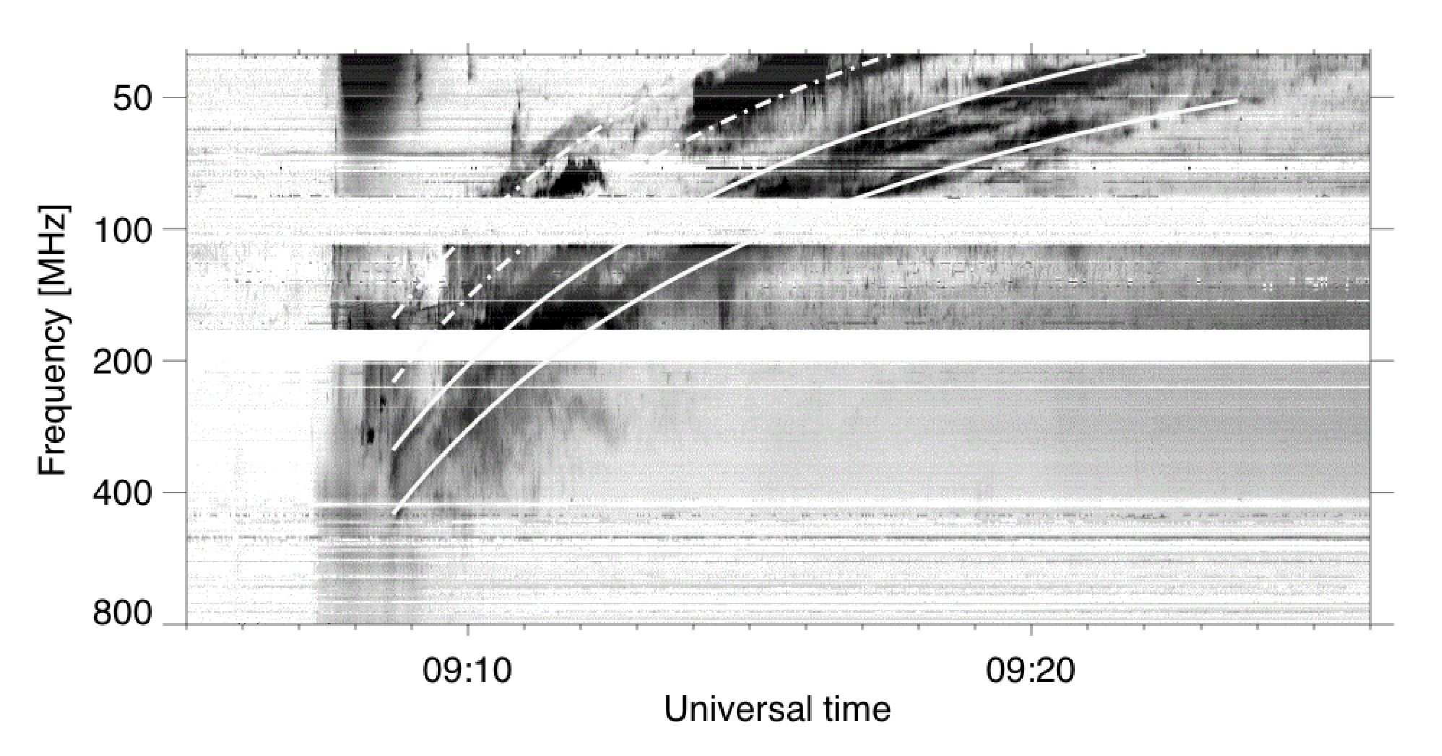
\includegraphics[trim=2cm 1cm 2cm 3cm, scale=0.25]{images/typeII}
\caption[Type II radio burst]{Type II radio burst observed at the Observatory Solar RadioAstronomy (OSRA) at Tremsdorf on 1997 November 3rd. Both the fundamental (dot-dash lines), and harmonic (solid lines) bands of emission are evident \citep{khan2002}.}
\label{fig:typeII}
\end{center}
\end{figure}

The development of radio instrumentation during and after the second world war presented scientists with the opportunity of (sometimes inadvertently) observing radio activity on the sun. Whilst performing radar tests using British military equipment, \citep{hey1946} reported a very high intensity radio source (10$^{7}$\,Jy) at 4-6 meters wavelength coming from the Sun. The relationship of these solar radio bursts with solar flaring activity was then reported by \citep{allen1947}. In the same year, \citet{payne1947} observed time series of single frequencies at 60\,MHz, 100\,MHz, 200\,MHz and noted that a delay in onset time of the burst from high to low frequency may suggest {\it \textquoteleft the excitation of radiation at successive levels by an agency traveling at finite velocity'}. %By assuming that the radiation is emitted at the $\tau=1$ layer for the observed frequency and using an empirical electron density formula for the corona, they deduced the speed of the 
%which they derived as 500-750\,km\,s$^{-1}$. They then noted that this is a similar velocity to the eruption of solar prominence material observed in the visible $-$ a remarkably accurate assertion given the fact they had no idea what caused the solar burst. 
The analysis of single frequency intensity time series was then superseded by the employment radiospectrographs to produce dynamic spectra of solar radio bursts. This allowed the identification of slowly drifting type IIs that are well characterized by modern radio-spectral observations. The hypothesis for the origin of these bursts was the same as that of \citet{payne1947} (a disturbance traveling into the corona at speeds of $10^{2}-10^{3}$\,km\,s$^{-1}$), except \citet{wild1954} correctly identified the emission to be generated at the frequency of plasma oscillation at the source height in the corona. \citep{uchida1960} and others eventually attributed these radio bursts to the activity that are they associated with today: type IIs are generated by magetohydrodynamic shocks transiting the corona. As the shocks propagate they excite radio emission at the local plasma frequency
\begin{equation}
\omega_p = \bigg( \frac{n_e e^2}{m_e \epsilon_0} \bigg)^\frac{1}{2}
\end{equation}
Since the plasma frequency is only dependent on electron number density, as the shock propagates to larger heights in the corona the frequency of emission drops owing to the dropping density. Hence the shock excites emission at decreasing frequency over time. This effect is further described in section 2.X
%-------------------- Asssociation with Flares -------------------------%

At the time Uchida and others made the assertion that type IIs were generated by MHD shocks, CMEs were as yet an undiscovered phenomena. Hence, the hypothesis that the origin of the shock was a flare-induced blast wave was a common one. The close onset times of flare maximum and type II onset supported this idea \citep{maxwell1962}. The association of type II radio bursts with a Moreton wave (a disturbance propagating away from flare site, observe in H-alpha), and the modeling of the two phenomena as a flare-induced explosive MHD disturbance gave credence to the idea that type IIs were indeed signatures of blast waves \citep{uchida1974}, a hypothesis later applied to type II observations \citep{kosugi1976}. 

%..however evidence in favor of the flare induced blast-wave could not explain the lack of correlation between between flare-size and type II occurence \citep{roberts1959, cliver 1999}.
%-------------------- Assocation with CMEs ---------------------------%
%\begin{figure}[!t]
%\begin{center}
%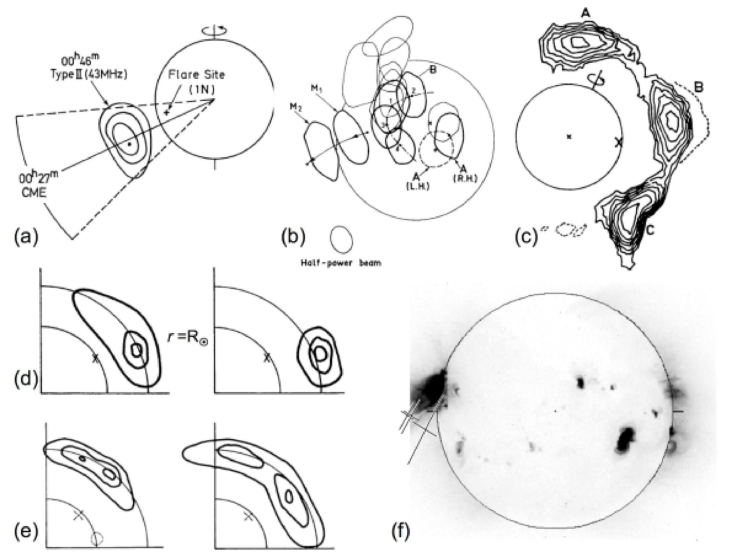
\includegraphics[ scale=1.1, trim=0cm 0cm 0cm 0.5cm]{images/typeII_sources.pdf}
%\caption{A compilation of observations of type II burst radio source. (a) 40\,MHz contours of a type II burst source region (Culogoora Radioheliograph) which was observed to be behind the leading edge of a CME (observed with SOLWIND) \citep{robinson1985}. (b) 80\,MHz contours of a type II radio burst sources (labelled B-1,2,3,4) observed with the Culgoora Radioheliograph. The sources labelled A are stationary type IV burst, while the M source are a moving type IV burst \citep{kai1969}. (c) 80\,MHz contours of the Culgoora radio heliograph showing multiple type II source (the whole extension is not once single type II source) \citep{smerd1970}. (d-e) 80\,MHz emission of type II radio burst source at a heliocentric distance of 1.6\,$R_{\odot}$, observed by the Culgoora Radioheliograph \citep{dulk1971}. (f) Sources of fundamental (164\,MHz), first (327\,MHz), and second harmonic (435\,MHz) of a type II radio burst observed by the Nan\c{c}ay Radioheliograph \citep{zlotnik1998}. Observation of second harmonic radiation is extremely rare.}
%\end{center}
%\label{fig:typeII_sources}
%\end{figure}
%TAKEN OUT TO REDUCE INTRO PAGES
\begin{figure}
\begin{center}
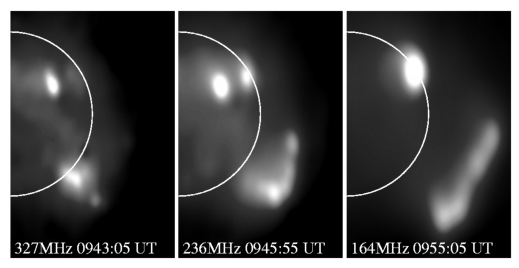
\includegraphics[scale=1.1, trim=0cm 0cm 0cm 0.5cm]{images/radio_shock.pdf}
\caption[Low frequency image of a radio shock]{Propagating radio emission source imaged at 327, 236, 164\,MHz using the Nancay Radioheliograph. The position of the emitting source is coincident with the CME leading edge \citep{maia2000}}
\label{fig:maia}
\end{center}
\end{figure}
Following the discovery of CMEs, the idea that mass motions (and not blast-waves) could produce type IIs came under consideration. Part of this idea came from the confirmation of the detection of in-situ shocks ahead of interplanetary CMEs, which were then called `plasma clouds' or `magnetic clouds' \citep{hundhausen1972}. Later, \citep{stewart1974} showed good correspondence of the height-time kinematics of a CME as observed by the coronagraph on OSO-7 and a type II burst source in images from the Culgoora Radioheliograph. This was taken as evidence that a piston-driven shock (CME-driven) was responsible for the type II. Following this was a statistical study that showed type II bursts to be highly associated with fast coronal mass ejections observed by the coronagraph on board Skylab \citep{gosling1976}. However, some doubts on the relationship were raised when \citep{robinson1985} showed that while 42\% of type IIs could be placed near the leading edge of a CME, some were located well behind the leading edge, this was considered to be evidence against the CME-driven shock idea. The CME hypothesis suffered another blow when
%The fact that some type IIs were associated with CMEs, while some seemed to be of blast wave origin was further elaborated upon in \citep{sheeley1984}. However, this could be a signature of a shock at CME flank Steinolfson
%(1985), a process asserted by more modern studies Vourlidas et al. (2003); Ontiverous and Mancuso 2010.
it was shown that of an observed 116 metric type II bursts, 45 had a clear association with CMEs and soft x-ray flares, but up to 19 were observed to occur without any associated CME. \citep{classen2002} later showed that type II burst onset times have been shown to occur up to more than one hour before CME onset time in some cases. The contradicting accounts of the association of CMEs with type IIs fueled a debate on which was the more reasonable explanation: are CMEs or flares more likely to drive a shock that causes type IIs?  
%Also, \citet{stein1985} has suggested that CMEs may drive shocks at their flanks.
%, a process asserted by white-light and multi-wavelength studies \citep{vourlidas2003, bemporad2010}.
%, while \citep{gopal2008} also revealed not all super-Alfvenic CMEs are accompanied by a type II burst. 
\begin{figure}[t!]
\begin{center}
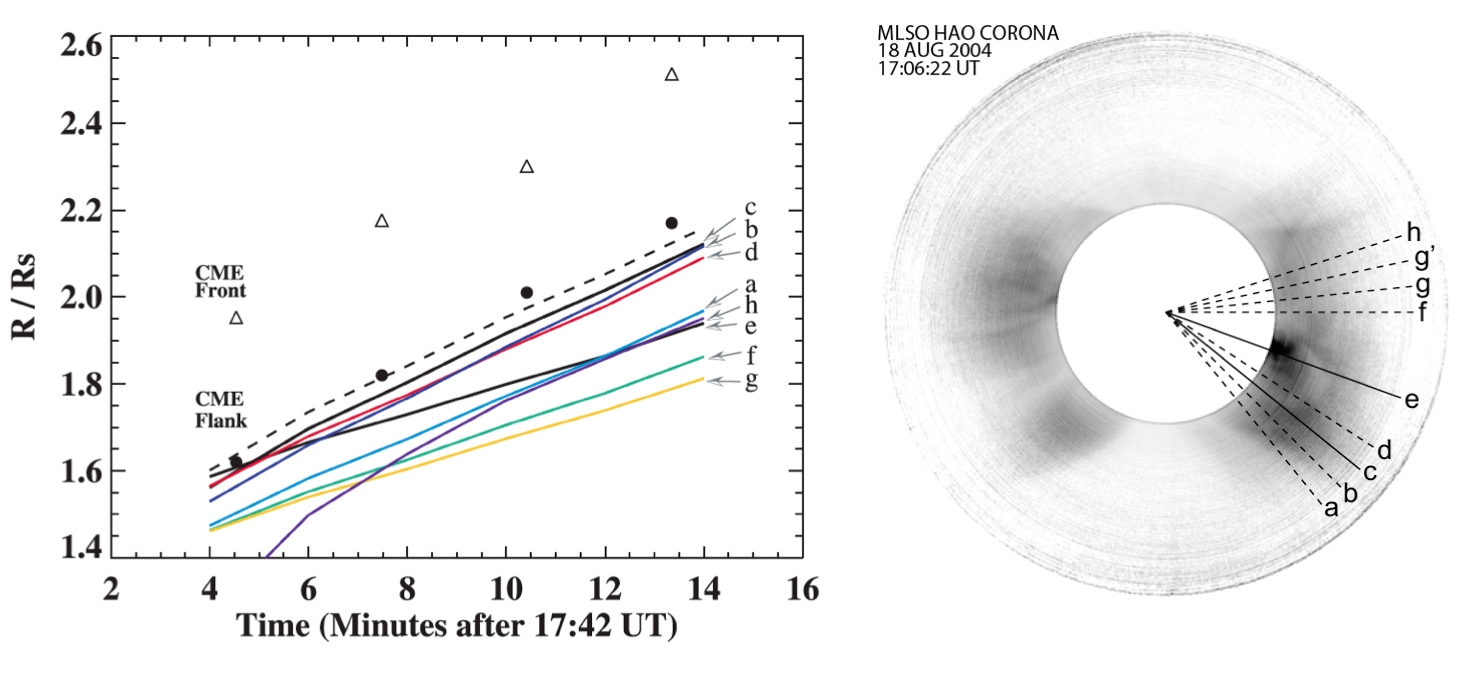
\includegraphics[scale=0.27, trim=0cm 1cm 0cm 1cm]{images/cho_trim.png}
\caption[Comparison of CME and type II height-time kinematics]{Comparison of height-time kinematics of a type II radio burst, observed using the Green Bank Solar Radio Burst Spectrometer (GBRBS), and CME as observed by the Mauna Loa coronagraph. Kinematics of CME at front an flank are shown, triangles and circles respectively.
Lines $a-h$ show the kinematics of the radio burst derived from density measurements performed along the trajectories (right panel). The CME and type II show the best match at the CME flank along trajectory $c$. Figure adopted \citep{cho2007}}
\label{fig:cho}
\end{center}
\end{figure}
Direct evidence of radio bright shocks have at least shown that CMEs are capable of driving the shocks \citep{maia2000} (Figure~\ref{fig:maia}).
In more recent times the debate continues, but the more sophisticated instrumentations, such as the Atmospheric Imaging Assembly, and multi-wavelength studies have offered a clearer picture. \citet{bain2012} has shown clear evidence of an erupting plasmoid with a type II radio source that sits at its nose, very direct evidence for CME driven type II. Material motions imaged at soft X-rays also suggest a driven shock \citep{klein1999}. Kinematics of the shock derived from the type II drift and position often show a good correspondence with CME kinematics \citep{mancuso2011}, however a statistical study by \citet{reiner2001}, shown in Figure~\ref{fig:reiner}, showed there to be little correlation between CME and type II speeds. This has been described as a discrepancy attributed to the shock possibly being located on the CME flank, the kinematics match better under this assertion \citep{mancuso2004} (Figure~\ref{fig:mancuso_kins}). \citep{cho2007, cho2012} has also shown that type II and CME kinematics match well when the shock is assume to be along the CME flank (Figure~\ref{fig:cho}). Later UV spectroscopic evidence that the flank-driven shock is indeed possible (Fig.~\ref{fig:mancuso_uv}). 

\begin{figure}[t!]
\begin{center}
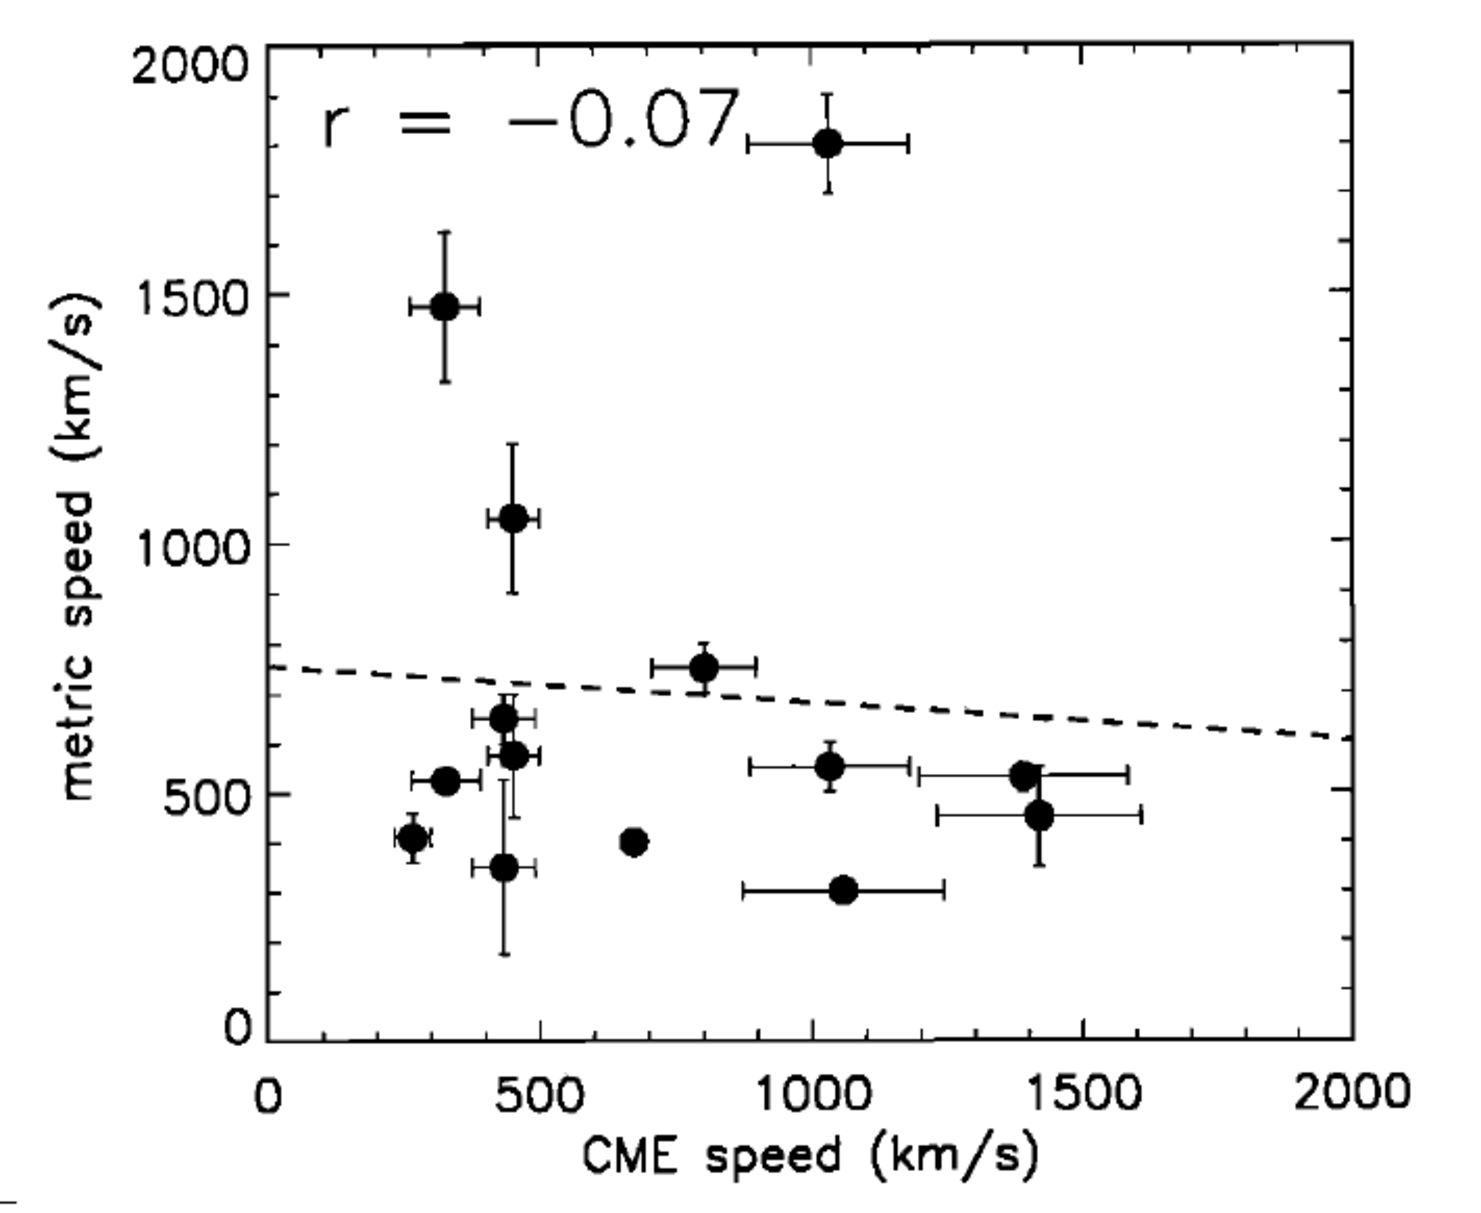
\includegraphics[trim=2cm 0cm 0cm 0cm, scale=0.3]{images/reiner2001.pdf}
\caption[Statistical comparison of CME and type II height-time kinematics]{A statistical comparison of metric type II speeds and CME speed \citet{reiner2001}. The two show no obvious relationship, taken to be evidence that a CME may not be the driver of the metric type IIs i.e., a CME was not responsible for the low coronal shock that caused these type IIs}
\label{fig:reiner}
\end{center}
\end{figure}

\begin{figure}[h!]
\begin{center}
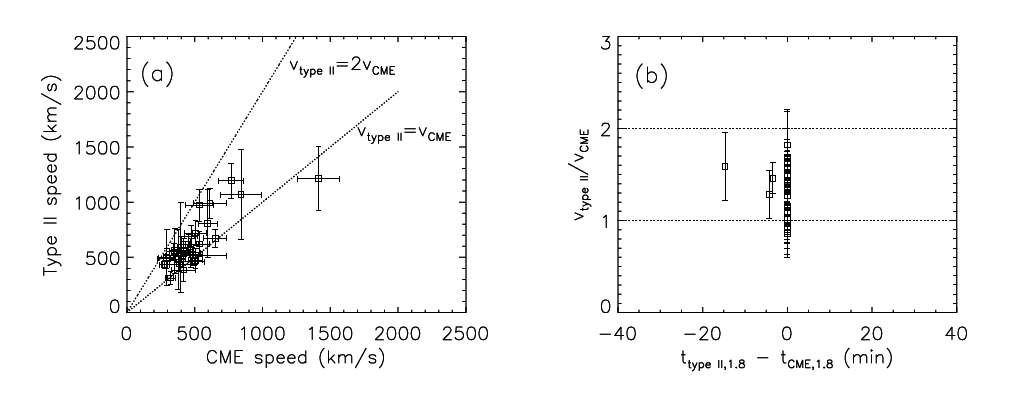
\includegraphics[trim=2cm 0cm 0cm 0cm, scale=0.45]{images/mancuso_kins2}
\caption[Comparison of CME and type II height-time kinematics, corrected for CME flank shock assumption]{Comparison of type II and CME kinematics taking into account that the type II may be along the CME flank, showing a much better correlation \citep{mancuso2004}.}
\label{fig:mancuso_kins}
\end{center}
\end{figure}

\begin{figure}[t!]
\begin{center}
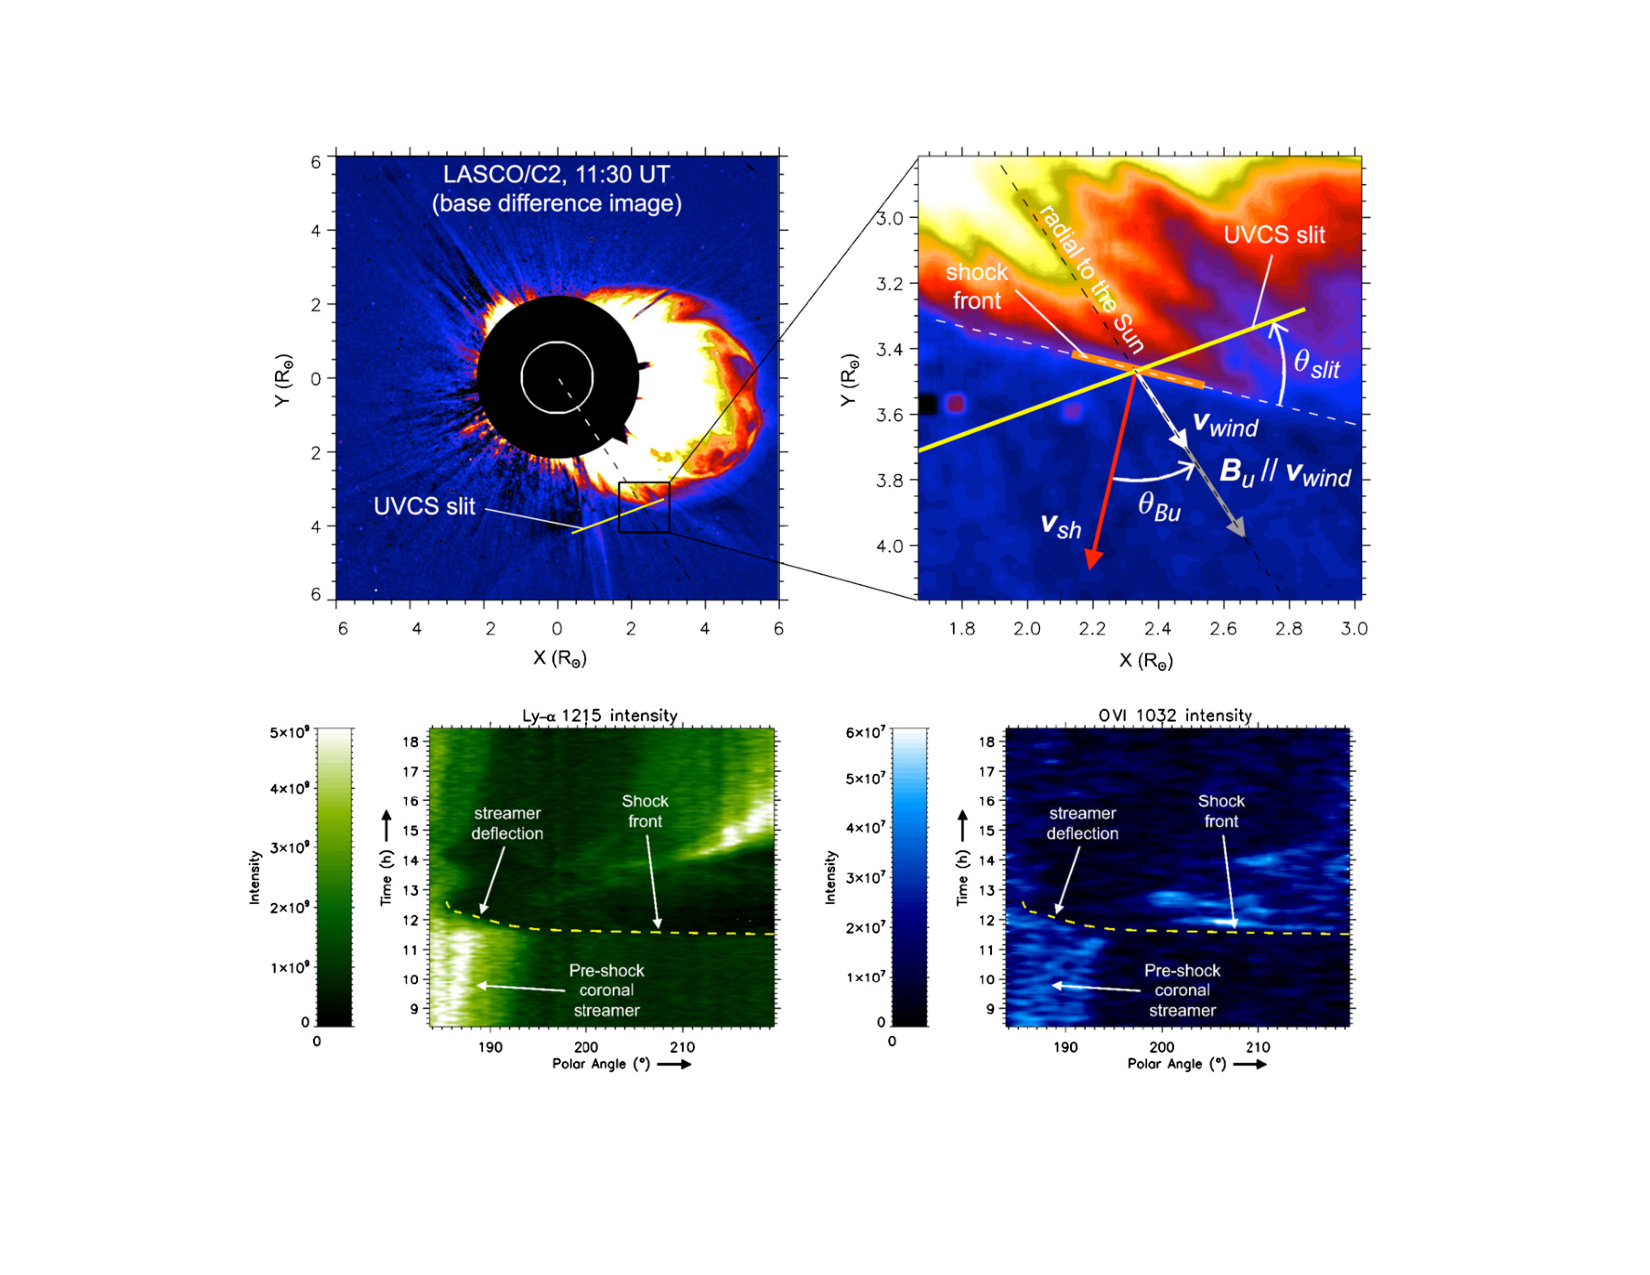
\includegraphics[trim=4.5cm 3cm 0cm 3cm, scale=0.75]{images/mancuso_uvcs.pdf}
\caption[CME flank shock observed by the UVCS spectrometer]{(Top) A LASCO C2 base-difference image of a CME on 2002 March 22, the yellow line marks the Ultraviolet Coronagraph Spectrometer (UVCS) slit located at CME flank. The event was associated with a type II radio burst. (Bottom) Space-time dependence of the H\,\Rmnum{1} Ly-$\alpha$ (left) and O\,\Rmnum{6} 1032\,\AA$~$(right) lines. The dashed yellow line shows the passage of the shock front. It results in a dimming of Ly-$\alpha$, caused by a deficiency in the resonant scattering of the line. This is due the scattering agent experiencing a bulk flow velocity that doppler shifts its absorption profile with respect to the incoming radiation, hence reducing its ability to scatter Ly-$\alpha$ efficiently$-$known as the Doppler dimming effect. The oxygen line, on the other hand, is collisionally controlled and depends on the ambient free electron density. As the shock transits it heats the plasma, resulting in more further free electrons and more efficient excitation of the O\,\Rmnum{6} 1032\,\AA, leading to brightening. The overall result is a dimming in the hydrogen line and a brightening of the oxygen line. This indication of bulk flow velocity as well as high levels of heating in the flow is evidence for a shock.}
\label{fig:mancuso_uv}
\end{center}
\end{figure}


Despite the fact that there is a large body of evidence for CME-driven shocks (at either the nose or flank) being associated with type IIs, there still remains convincing studies on the blast-wave possibility. \citet{vrsnak2000a,vrsnak2000b} has formulated an analytical model to describe the blast-wave generation of type IIs. The analytical treatment shows the fast onset times ($>10$\,min) of type IIs after flare start cannot be account for by CME eruption \citep{vrsnak2001}. The most recent direct evidence was given by \citep{mag2012}, when they showed a compact flare with no sign of any eruption in h$\alpha$, EUV or white-light imaging. The debate rages on, and there is no consensus on either CME-driven shocks or flare-ignited blast waves \citep{vrsnak2008} \footnote{It should be noted there is no ambiguity on the nature type IIs in the hecto-kilometric range. The accepted paradigm for these type IIs is a shock driven by a CME at interplanetary distances which may then be detected in situ as a shock. However, another controversy stemming from the flare-driven/CME-driven argument for type IIs is whether interplanetary type IIs and low coronal type IIs belong to the same driver \citep{cane2005}.}.

%Goplswamy 2005, CME energies and type II correlation. Also shows height of CMEs at onset time of type II. 
%http://adsabs.harvard.edu/abs/2009SoPh..259..227G also shows start time of type IIs relative to CME h-t
%\footnote{It should be noted that the debate only concentrates on metric type IIs i.e., those that occur on the low corona. Decametric-kilometric type IIs are now well established to be the result of shocks driven by interplanetary CMEs.}.

%It should be noted there is no ambiguity on the nature t ype IIs in the hecto-kilometric range. The accepted paradigm for these type IIs is a shock driven by a CME at interplanetary distances which may then be detected in situ as a shock. However, another controversy stemming from the flare-driven/CME-driven argument for type IIs is whether interplanetary type IIs and low coronal type IIs belong to the same driver \citep{cane2005}.

Finally, a part of the controversy with determining the source of all radio bursts (not just type II) is to do with the the method by which radio burst kinematics are deduced from density models of the solar atmosphere. The models can often lead to questionable kinematics and heights of the radio sources, as discussed in Section~\ref{sec:freq_drift}
%For the majority of cases, an attempt is made to derive the height from which radio burst was generated. This is done by assuming that the radio emission is plasma radiation (generally a sound assumption), allowing a direct conversion from plasma frequency to electron density of the environment from which the emission came. Since the coronal is in general a gravitationally stratified medium, the density will be associated with a particular height. In the simplest case we may treat the corona as being in hydrostatic equilibrium, using a density scale height to estimate how density varies as a function of distance from the solar surface. However, a more popular method is via the use of semi-empircal density models usually those Newkirk, Saito, Baunbach Allen, amongst many others. The use of these models allows an estimate of the height from which the burst originated. However, the models are very general description of the corona and do not take into account that this region of the solar atmosphere can be very dynamic, changeable over periods of hours, and quite inhomogeneous. The models in no way account for this, and, as a result, they may provide a very erroneous estimation of the radio burst height as well as providing an unreliable estimate of any derivative properties such as speed of the radio burst. It is not surprising that the speeds of type IIs are not reliable when derived via density models. A further discussion of this is given in Appendix X.
% Cho has some great papers about type IIs and shocks at the CME flank

%----------------------------- Herringbones --------------------------------%
\subsection{Herringbones and Type IIIs}

As will be shown in Chapter 2, radio burst such as type IIs are believed to be the result of a plasma instability in the presence of high velocity electron beams. There is a subset of type II radio bursts which directly observe the electron beam nature of these radio bursts, known as `herringbone' radio bursts as shown in Figure~\ref{fig:herringbones} \citep{cairns1987, cane1998}. These are the signature of bursty electron acceleration occurring at a coronal shock front \citep{mann2005}. The herringbone spike is an individual beam of electrons traveling away from the shock. 

The fact that they drift towards both low and high frequencies simultaneously means they are bi-directional in space e.g., drifting toward and away from the sun simultaneously. The `bursty' or quasi-periodic nature of the herringbones occurs over timescales of seconds \citep{mann1995, mann2005} and they are believed to be a result of the shock drift acceleration (SDA) process \citep{miteva2007}. The burstiness has been suggested to be due to inhomogeneity on the shock front, and may be signature of a so-called `wavy' or `rippled' shock front \citep{zlobec1993, guo2010, vandas2011}. This means they provide a measure of shock structure and a timing of the particle acceleration process itself. The bursts are rare, with only 20\% of type II bursts exhibiting these structures \citep{cairns1987}. Thus a complete theory on their formation does not exist. They have been attributed to shocks propagating parallel to the solar surface (tangentially across radial field lines) whereby \textquoteleft shock fronts propagate normal to the magnetic field and continuously eject bunches of fast electrons long the field' (verbatim from \citet{wild1964}); this assertion was also illustrated in \citet{stewart1980}. Such a mechanism could occur if the CME flank drove a shock transversely through the corona (parallel to the solar surface). An alternative theory is one where the herringbones are produced in the termination shocks of super-Alfv\'{e}nic outflow jets of a reconnection region \citep{aurass2002, aurass2004}. Such a process could be the result of a reconnection region in a current sheet in the wake of a CME, as described by the standard solar flare model. The rarity of herringbone observations has resulted in no consensus on how they might be produced, and their formation mechanism remains unconfirmed.
\begin{figure}[!t]
\begin{center}
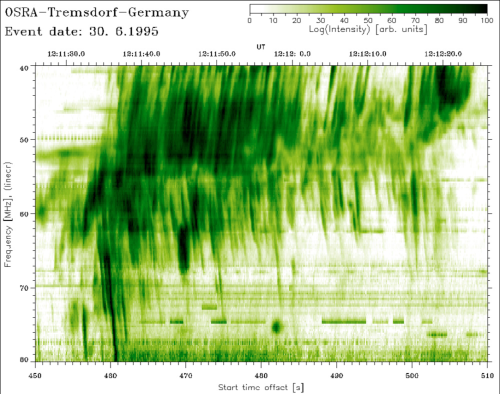
\includegraphics[scale=1.4]{images/miteva_herbones.pdf}
\caption[Herringbone radio bursts]{Fine structure observed in a type II radio burst known as \textquoteleft Herringbones'. Each spike is an individual beam of electrons accelerated away from the coronal shock. The presence of herringbones drifting to both low and high frequencies is indicative of electron beams traveling toward and away from the Sun.}
\label{fig:herringbones}
\end{center}
\end{figure}

Related to particle accelerations in the corona are type III radio bursts. These are fast drifting features in dynamic spectra ($\sim$20\,MHz\,s$^{-1}$) and are the characteristic radio signature of electrons beams traveling on open magnetic field lines in the corona \citep{pick2008}. Type IIIs are mainly associated with an acceleration process directly from the flaring active region e.g., acceleration directly out of the reconnection process. However, some type IIIs are thought to be associated with the in-situ detection of shock accelerated electrons. Indeed sometimes type II shock signatures are seen to occur with type IIIs, an indication of electron acceleration from the shock $-$ these type IIIs are sometimes labelled \textquoteleft shock-associated' or SA type IIIs \citep{bougeret1998}. In certain instances the particle acceleration as indicated by type III bursts has been related to shock feature seen the corona. This is usually in the context of coronal bright front studies.

\subsection{Coronal Bright Fronts}
%------------------- CBFs, type IIIs, herringbones, and SEPs -------------------------------%
As mentioned, some of the explanations as to why a type II source may appear behind the CME front was the possibility of a shock driven by the CME flanks. As well as this, certain studies of type III radio burst associated with in-situ detection of solar energetic particles have been related to some shock driver low in the corona. One possible observational signature of shock activity in the low corona is a coronal bright front (CBF), also known as an \textquoteleft EUV wave'.
\begin{figure}[!t]
\begin{center}
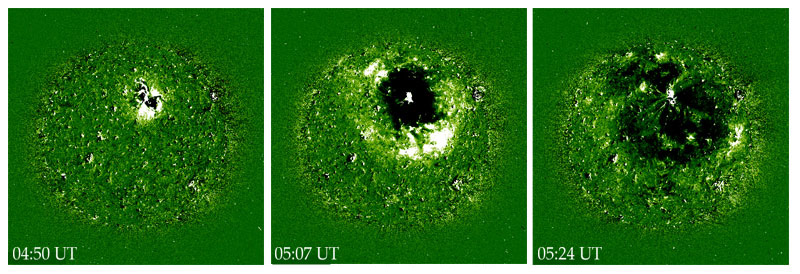
\includegraphics[scale=0.5, trim=0cm 0cm 0cm 1cm]{images/eit_19970512_wave}
\caption[First observation of an \textquoteleft EIT wave']{One of the first observed coronal bright fronts, reported by \citep{thompson1998}. The images are EIT \,\AA\, base differenced so the bright front can be seen expanding across the solar disk. This bright front is postulated to be a magnetohydrodynamic wave propagating in response to an eruptive event in the solar corona.}
\label{fig:cbf}
\end{center}
\end{figure}

CBFs were discovered in 1997-1998 \citep{moses1997, thompson1998} by the EIT instrument on SOHO (they are sometimes called \textquoteleft EIT waves'). CBFs are are bright fronts imaged at EUV and observed to propagate from an eruptive active at typical speeds of between 200-400\,km\,s$^{-1}$ \citep{thompson2009}. Given their speed of propagation and their tendency to undergo reflection \citep{gopal2009}, refraction \citep{wang2000}, and pulse broadening \citep{long2011}, there is a prevailing hypothesis that these features are fast mode magnetohydrodynamic waves propagating through corona \citep{veronig2010}.
\begin{figure}[!t]
\begin{center}
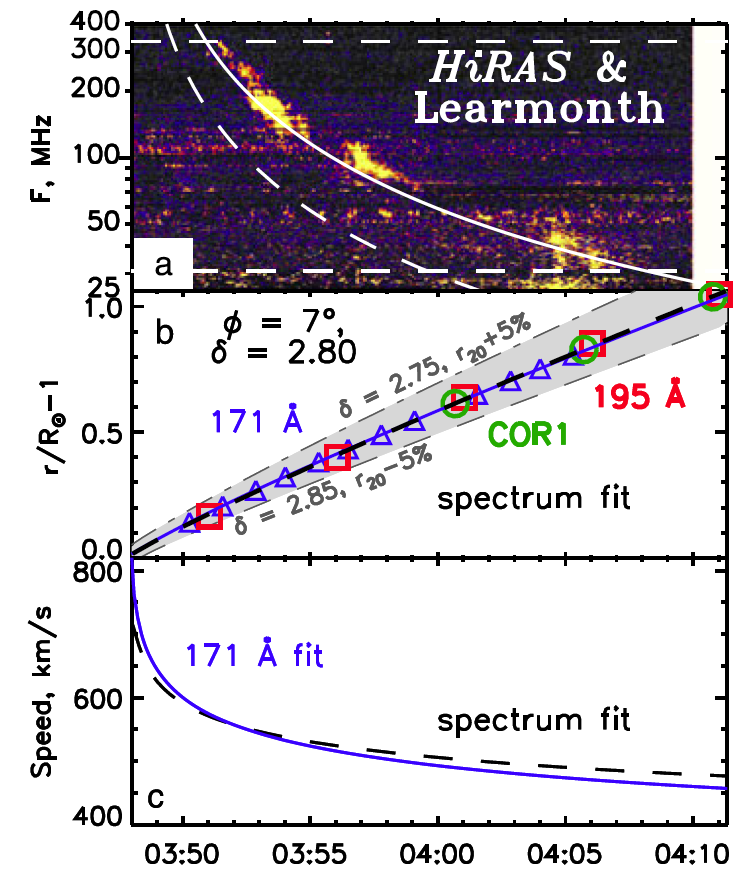
\includegraphics[trim=3cm 0cm 0cm 2cm, scale=0.3]{images/grechnev2011}
\caption[Comparison of EUV wave and type II height-time]{Top: Type II radio burst observed by the HiRAS spectrograph at Learmonth, Australia. Middle: Coronal bright front height time measurements from EUVI 195\,\AA\, (red squares), 171\,\AA\,(blue triangles), and COR1 (green circles). Fit to the type II burst converted to height is shown by the dashed black line. The type II burst height-time perfectly matches the eruption of the CBF as seen by EUVI and CME as seen by COR1 \citep{grechnev2011a}}
\label{fig:typeII_cbf}
\end{center}
\end{figure}
They are known to accompany CME eruption quite closely \citep{bieseker2002}, so it is thought that a CME may be their driver i.e., as the CME expands it drives a disturbance through the corona which manifests itself as bright front in EUV images. Like CME eruption, CBFs show a clear association with type II radio bursts, with up 90\% of type IIs being associated with CBFs \citep{klassen2000}. The fact that this MHD wave-like phenomena shows a clear association with an MHD shock signature prompted the interpretation that they belong to the same MHD disturbance in the corona \citep{warmuth2004b}, both driven by a CME. Indeed, type II kinematics can sometimes show a very closely correspondence with CBF kinematics \citep{vrsna2005, grechnev2011} (Figure~\ref{fig:typeII_cbf}). Also, CBFs images at EUV may also have a counterpart images at soft X-ray (SXR) with a type II closely tied to the event e.g., the type II burst in Fig.~\ref{fig:typeII} showed such a relationship with SXR activity \citep{khan2002}


To further this hypothesis, there area number of studies which suggest that the origin of in-situ detection of SEPs, and the type III bursts they are associated with, have their origin in the same disturbance responsible for the CBF \citep{klassen2002, krucker1999, kozarev2011}. The idea naturally leads to the following physical scenario: the CME eruption drives a pressure pulse, observable in the low corona as a propagating CBF; this scenario is modeled in Figure~\ref{fig:shock_cbf}. Higher in the corona this same pulse forms a shock, accelerating particles and producing type II. If this shock encounters open magnetic field lines it may accelerate particles along the open field, producing type III emission and the possible subsequent detection of in-situ SEPs. Hence the unifying theme amongst the CME, CBF, radio burst, and accelerated particles is a CME driven shock.
\begin{figure}[!t]
\begin{center}
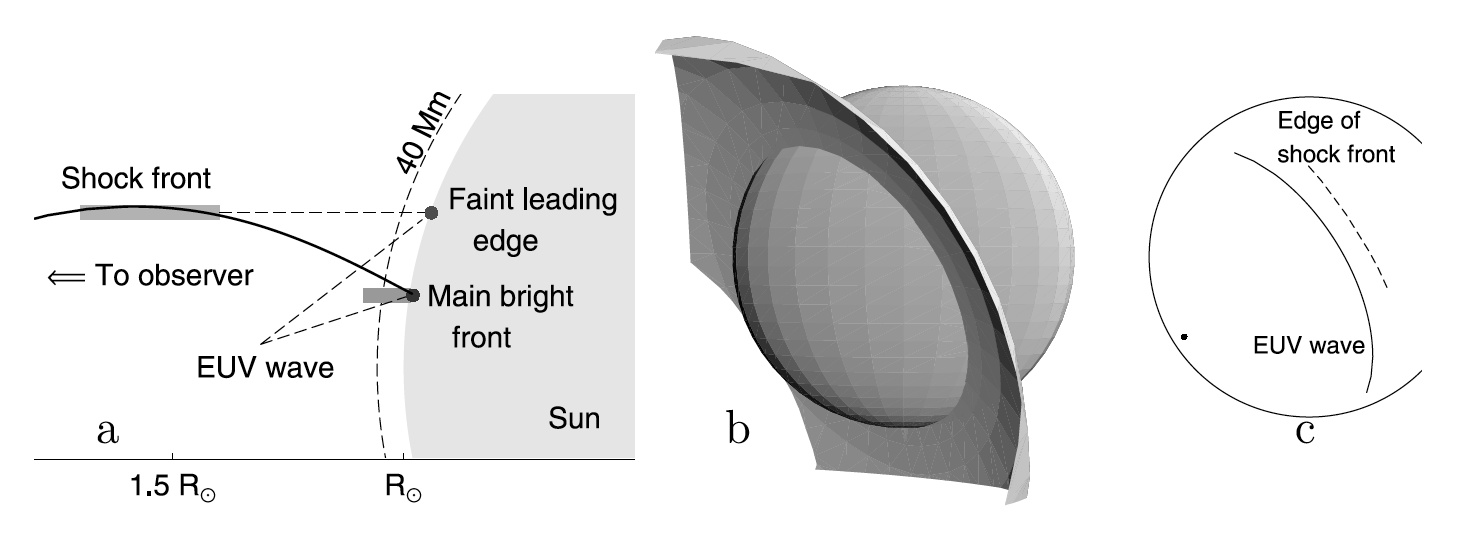
\includegraphics[scale=0.25, trim=1cm 0cm 0cm 2cm]{images/shock_sim}
\caption[Model of EUV wave and coronal shock]{Model of a coronal disturbance resulting in a CBF in the low corona, and a steepening into a shock higher in the corona \citep{grechnev2011a}.}
\label{fig:shock_cbf}
\end{center}
\end{figure}

However, such a mechanism may be called into doubt, given that CBFs can often display kinematics that may not be explained by a wave. This has prompted a `pseudo-wave' interpretation, whereby the erupting CME produces a large-scale restructuring or reconnecting of coronal magnetic field \citep{chen2002, attrill2007}. The bright front may also be due to current shell around the CME as it encounters the coronal field during eruption, this may result in a bright pulse via Joule plasma heating that is not actually a driven wave \citep{delannee2008}. In this scenario, any relationship with shock observables is indirect, and the relationship with the particle acceleration process may be brought about by magnetic reconnection, such as interchange reconnection at the flanks of a CME \citep{maia2004}. Hence it is not clear how close the relationship of CBFs is to the many shock observables in the corona e.g., is the CBF a low-coronal, low-amplitude counterpart of a shock front higher in the corona? Are radio bursts and particle acceleration in any way associated with this shock front? Does the CME drive this shock front? Despite a close temporal correspondence between CMEs, radio bursts and CBFs, the shock wave link between these phenomena has not been definitively proven or discredited.

\subsection{White-light Shocks}

There is a wealth of evidence in radio and ultraviolet to suggest the transit of CME driven shocks in the corona. Some of this evidence suggests that these shocks may occur at the CME flank as well as ahead of its apex. It has been shown in some studies that these shocks may be directly imaged in white-light coronagraph images \citep{vourlidas2012, vourlidas2013}. Under high contrast a much fainter front may be seen ahead of the main front, four such events are shown in Figure~\ref{fig:wl_shock}. 
\begin{figure}[!t]
\begin{center}
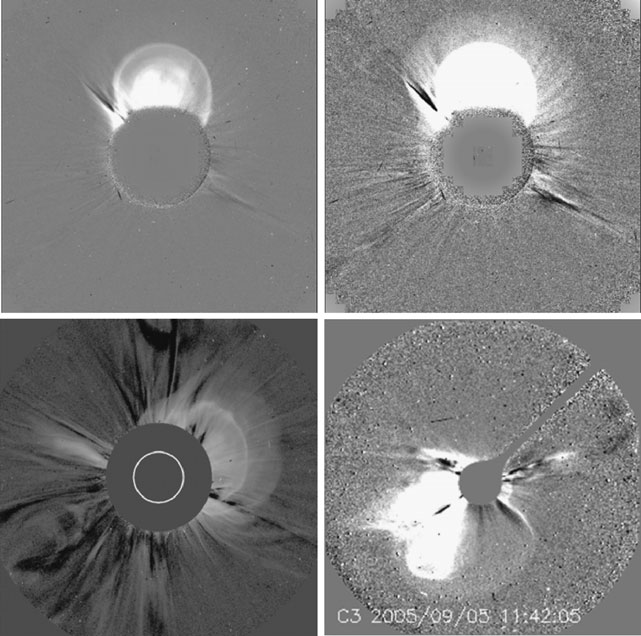
\includegraphics[scale=0.9, trim=0cm 0cm 0cm 0.5cm]{images/wl_shock.pdf}
\caption[White-light image of shocks]{Coronal mass ejections displaying evidence of shocks. The much fainter secondary front is a candidate for a CME driven shock \citep{vourlidas2013}}
\label{fig:wl_shock}
\end{center}
\end{figure}
This `two-front' morphology is a common occurrence in white-light CME structure and constitutes a reliable signature of a CME front followed by a stand-off shock \citep{vourlidas2013}. In many instances they have been used as qualitative confirmation for the presence of a CME-driven shock in the corona. Indeed, it has been used to identify shock candidates at the flank of a CME \citep{vourlidas2003}. However, some studies have inferred various quantitative shock parameters such as the compression ratio \citep{ontiveros2009}, or by considering the shock geometry. Stand-off shocks are a common occurrence in nature and their theoretical development in an astrophysical context has been applied to planetary magnetospheric bow shocks whereby the radius of curvature of the driver and the stand-off distance between the nose of the driver and the bow shock may allow a calculation of the Mach number \citep{spreiter1966}. This applies to shocks on all physical scales, from bullets and aircraft, to planetary magnetospheres and CMEs \citep{russel2002}. In its application to CMEs, the theory was used to derive coronal magnetic field \citep{kim2012}, shock Mach numbers in the low corona \citep{gopal2012}, as well as Mach numbers in the outer corona as far as $\sim0.5\,A.U.$ \citep{maloney2011}. 

% Put in any studies got to do with white-light shocks and type II observation. Where possible, also put in studies of white-light shocks and CBFs.


%\begin{itemize}
%\item Association of type IIs with CMEs. Herringbones and particle accelerations
%\item Association of type IIs with CMEs
%\item Radio imaging of shocks
%\item Relationship to EUV waves, Moreton waves
%\item Shocks at other wavelengths
%\item The importance of multi-wavelength studies
%\end{itemize}

\section{Thesis Outline}

The work in this thesis firstly advances the understanding of CME masses, energies and forces. As outlined above, very few observational studies of CME masses exist, and CME energy studies a fewer still. Almost no observational studies of CME forces exist. The reason for this is that, to date, CME masses and dynamics observations have been severely hindered by the very large uncertainties in CME mass. This has been due to the unknown propagation direction and width of the CME, making a determination of the uncertainties on the mass impossible. Very uncertain masses combined with equally uncertain kinematics has lead to virtually no quantification of the total force acting on CMEs as they propagate. This thesis will address this issue by showing that CME mass and energies may be quantified more reliably and with much reduced uncertainty when the dual vantage points of the STEREO spacecraft are used. Also, for the first time in the field, an observational quantification of the forces acting on CMEs will be presented. 

Secondly, this thesis will outline the behavior of CMEs and radio bright shocks in the low corona. Up until now, the relationship between CME, CBFs, and radio bursts has remained unknown. It is not known whether CMEs dive shocks through the corona, the low coronal manifestation of which is a CBF. It is also undetermined if the radio bursts are generated in this same wave/shock system. This work will show that the relationship between CMEs, CBFs, and radio bursts is a plasma shock. Furthermore, it will show that this shock was driven by the expansion of the CME flank, and was responsible for bursty particle acceleration.

Chapter 2 will first discuss MHD, CME theory and related phenomena. Secondly it will discuss the plasma shock theory that is relevant to this study i.e., the MHD Rankine-Hugoniot relations, shock particle acceleration, and radio burst generation. Chapter 3 will discussed the variety of instrumentation used in this study, including the installation of the Rosse Solar Terrestrial Observatory (RSTO). Chapter 4 involves the CME masses, kinematics and dynamics work, while Chapter 5 will discuss the CME, CBF, radio bursts and plasma shock work. Chapter 6 will summarise the main findings and conclusions of this thesis and present the future direction of the study.
